\documentclass[LSR, MA, english, intermediate]{LSR_thesis} 
\graphicspath{{pics/}}

%% Options:
%% LSR: LSR Template with Prof. Buss as default
%% ITR: ITR Template with Prof. Hirche as default

%% BA: Bachelorarbeit / Bachelor thesis
%% MA: Masterarbeit / Master thesis
%% HS: Hauptseminar / Scientific seminar
%% PP: Projektpraktikum / practical course
%% IP: Ingenieurpraxis
%% FP: Forschungspraxis
%% SeA: Semesterarbeit (MW)

%% english
%% german

%% final
%% intermediate

%% tutorial -> remove flag such that help files and todos are removed

%%________________________________________________%
%%_________CUSTOMIZE LATEX ONLY IN customize.tex!_% 
%%_________ DO NOT MODIFY THE TEMPLATE!___________%
%%________________________________________________%
%% add customize first so you can access your commands in gloss
%%%%%%%%%%%%%%%%%%%%%%%%%%%%%%%%%%%%%%%%%%%%%%%%%%%%%%%%%%%%%%
% CUSTOMIZING Tex-File for students to be adjusted as needed %
%%%%%%%%%%%%%%%%%%%%%%%%%%%%%%%%%%%%%%%%%%%%%%%%%%%%%%%%%%%%%%
%%%%%%%%%%%%%%%%%%%%%
% CUSTOM PACKAGES	%
%%%%%%%%%%%%%%%%%%%%%
\usepackage{tikz}
\usepackage{pgfplots}

% \usepackage{IEEEtrantools}

%%%%%%%%%%%%%%%%%%%%%
% CUSTOM COMMANDS	%
%%%%%%%%%%%%%%%%%%%%%
% e.g. Math conventions as vectors, Matrices, sets
\renewcommand{\vec}[1]{\mathbf{\MakeLowercase{#1}}}
\newcommand{\Mat}[1]{\mathbf{\MakeUppercase{#1}}}
\newcommand{\set}[1]{\boldsymbol{#1}}

% e.g. use differenc layers in tikz
\pgfdeclarelayer{background}
\pgfdeclarelayer{nodelayer}
\pgfdeclarelayer{edgelayer}
\pgfdeclarelayer{foreground}
\pgfsetlayers{background,edgelayer,nodelayer,main,foreground}
%%%%%%%%%%%%%%%%%%%%%
% HYPHENATIONS 		%
%%%%%%%%%%%%%%%%%%%%%
\hyphenation{Lya-pu-nov}

 % add custom commands etc in this file 
% %%%%%%%%%%%%%%%%%%%%%%%%%%%%%%%%%%%%%%%%%%%%%%%%%%%%%%%%%%%%%%
% NOTE: Using this is optional.
% 	Nonetheless, feel free to include this file and adjust the 
% 	examples below as needed.
%   
%
% Further reading:
%	https://ctan.org/pkg/glossaries?lang=en
%%%%%%%%%%%%%%%%%%%%%%%%%%%%%%%%%%%%%%%%%%%%%%%%%%%%%%%%%%%%%%


% include packages
\usepackage[acronyms, style=alttree, toc=true, nonumberlist, nogroupskip, nopostdot, automake]{glossaries}

%%%%%%%%%%%%%%%%%%%%%%%%%%%%%%%%%%
% DEFINE HEADINGS AND CATEGORIES %
%%%%%%%%%%%%%%%%%%%%%%%%%%%%%%%%%%
\newcommand{\Notation}{Notation}
\newcommand{\Symbols}{List of Symbols}

\newglossary{notation}{not}{nt}{\Notation}
\newglossary{symbols}{sym}{sbl}{\Symbols}

\glssetwidest{THISWIDE} % adjust width of glossary

\makeglossaries

%===========%
% ACRONYMS	%
%===========%
\newacronym{MPC}{MPC}{model-predictive control}
\newacronym{BIBO}{BIBO}{bounded-input bounded-output}
\newacronym{HRC}{HRC}{human-robot collaboration}

%============%
% SYMBOLS	%
%===========%
\newglossaryentry{control}{type=symbols,
	sort={control},
	name={\ensuremath{\vec{u}}},
	description={control input vector}
}
\newglossaryentry{uk}{type=symbols,
	sort={control},
	name={\ensuremath{\vec{u}_k}},
	description={control input vector with time step}
}

\newglossaryentry{xk}{type=symbols,
	sort={state},
	name={\ensuremath{\vec{x}_k}},
	description={state vector with time step}
}

%============%
% NOTATION	%
%===========%
\newglossaryentry{vector}{type=notation,
	sort={vector},
	name={\ensuremath{\vec{x}_n}},
	description={$n$-dimensional vector named $x$}
}	

\newglossaryentry{matrix}{type=notation,
	sort={vector-matrix},
	name={\ensuremath{\Mat{x}_{m\times n}}},
	plural={matrices},
	user1={Mat},
	description={\ensuremath{m\times n} dimensional matrix  named \ensuremath{X}}
}

\glsaddall % Print all glossary entries

%%%% Add GLOSSARIES at end of thesis
\newcommand{\AddMyGloss}{
	\cleardoublepage
   	\printglossary[type=acronym, nogroupskip]
	
	\ifdefined\Notation
		\cleardoublepage
		\printglossary[type=notation, nogroupskip]
	\fi
	
  	\ifdefined\Symbols
  		\cleardoublepage
		\printglossary[type=symbols, nogroupskip]
	\fi
}

		% add your glossary in this file 


%% start document
\begin{document}

%%%%%%%%%%%%%%%%%%%%%%%%%%%%%%%%%%%%%%%%%%%%%%%%%%%%%%%%%%%%%%%
%%%%%%%%%%%%%%%%%%% Title Page %%%%%%%%%%%%%%%%%%%%%%%%%%%%%%%%
%%%%%%%%%%%%%%%%%%%%%%%%%%%%%%%%%%%%%%%%%%%%%%%%%%%%%%%%%%%%%%%
%% English title:
\title{Kernel Embedding for Particle Gibbs-Based Optimal Control}

%% German title (for German theses only)
%\title{Die Antwort auf Alles und Mehr - Ein Trauerspiel in 4 Akten}
% and English translation (optional)
\titletranslation{
%Die Verwendung eines Deutschen Untertitels obliegt der Verantwortung der entsprechenden Betreuer
}

%% insert your data here:
\student{Lukas Hochschwarzer} % your name
%\studtitle{} % your title
\street{Koenigswieser Strasse 75e} % your address
\city{81475 Munich} % postal code and city
\phone{089 - 1015332} % your telephone number

 
%-if more students are involved (e.g., PP)-
%\studenttwo{Second Student}
%\studtitletwo{} 
%\studentthree{} 
%\studtitlethree{} 
%\studentfour{} 
%\studtitlefour{} 
%-----------------------------------------

\supervisor{M.Sc. Robert Lefringhausen} % your supervisor
\finalrep{XX.XX.2024} % submission date

\maketitle

%%%%%%%%%%%%%%%%%%%%%%%%%%%%%%%%%%%%%%%%%%%%%%%%%%%%%%%%%%%%%%%
%%%%%%%%%%%%%%%%%%% Second Page %%%%%%%%%%%%%%%%%%%%%%%%%%%%%%%
%%%%%%%%%%%%%%%%%%%%%%%%%%%%%%%%%%%%%%%%%%%%%%%%%%%%%%%%%%%%%%%
\newpage
\cleardoublepage
\ifLSRITRtutorial
		\phantom{u}
		\phantom{1}\vspace{6cm}
	\begin{center}
		\add[inline]{In your final hardback copy, replace this page with the signed exercise sheet.}
		\vspace{3cm}
		\add[inline]{!! If you delete this page, make sure that the page structure is maintained !!
		
		(when printed, (even) page numbers on \textit{left pages} must be on the left side, (odd) page numbers on \textit{right pages} on the right side}
		\vspace{3cm}
		\todo[inline,color=red!70]{Before modifying this document, READ THE INSTRUCTIONS AND GUIDELINES!
		
		(remove \textit{tutorial} flag in the first line of this file to remove template tutorial parts)}
	\end{center}
\else
	% in case you want to add the PDF directly add the task description in the include directory
	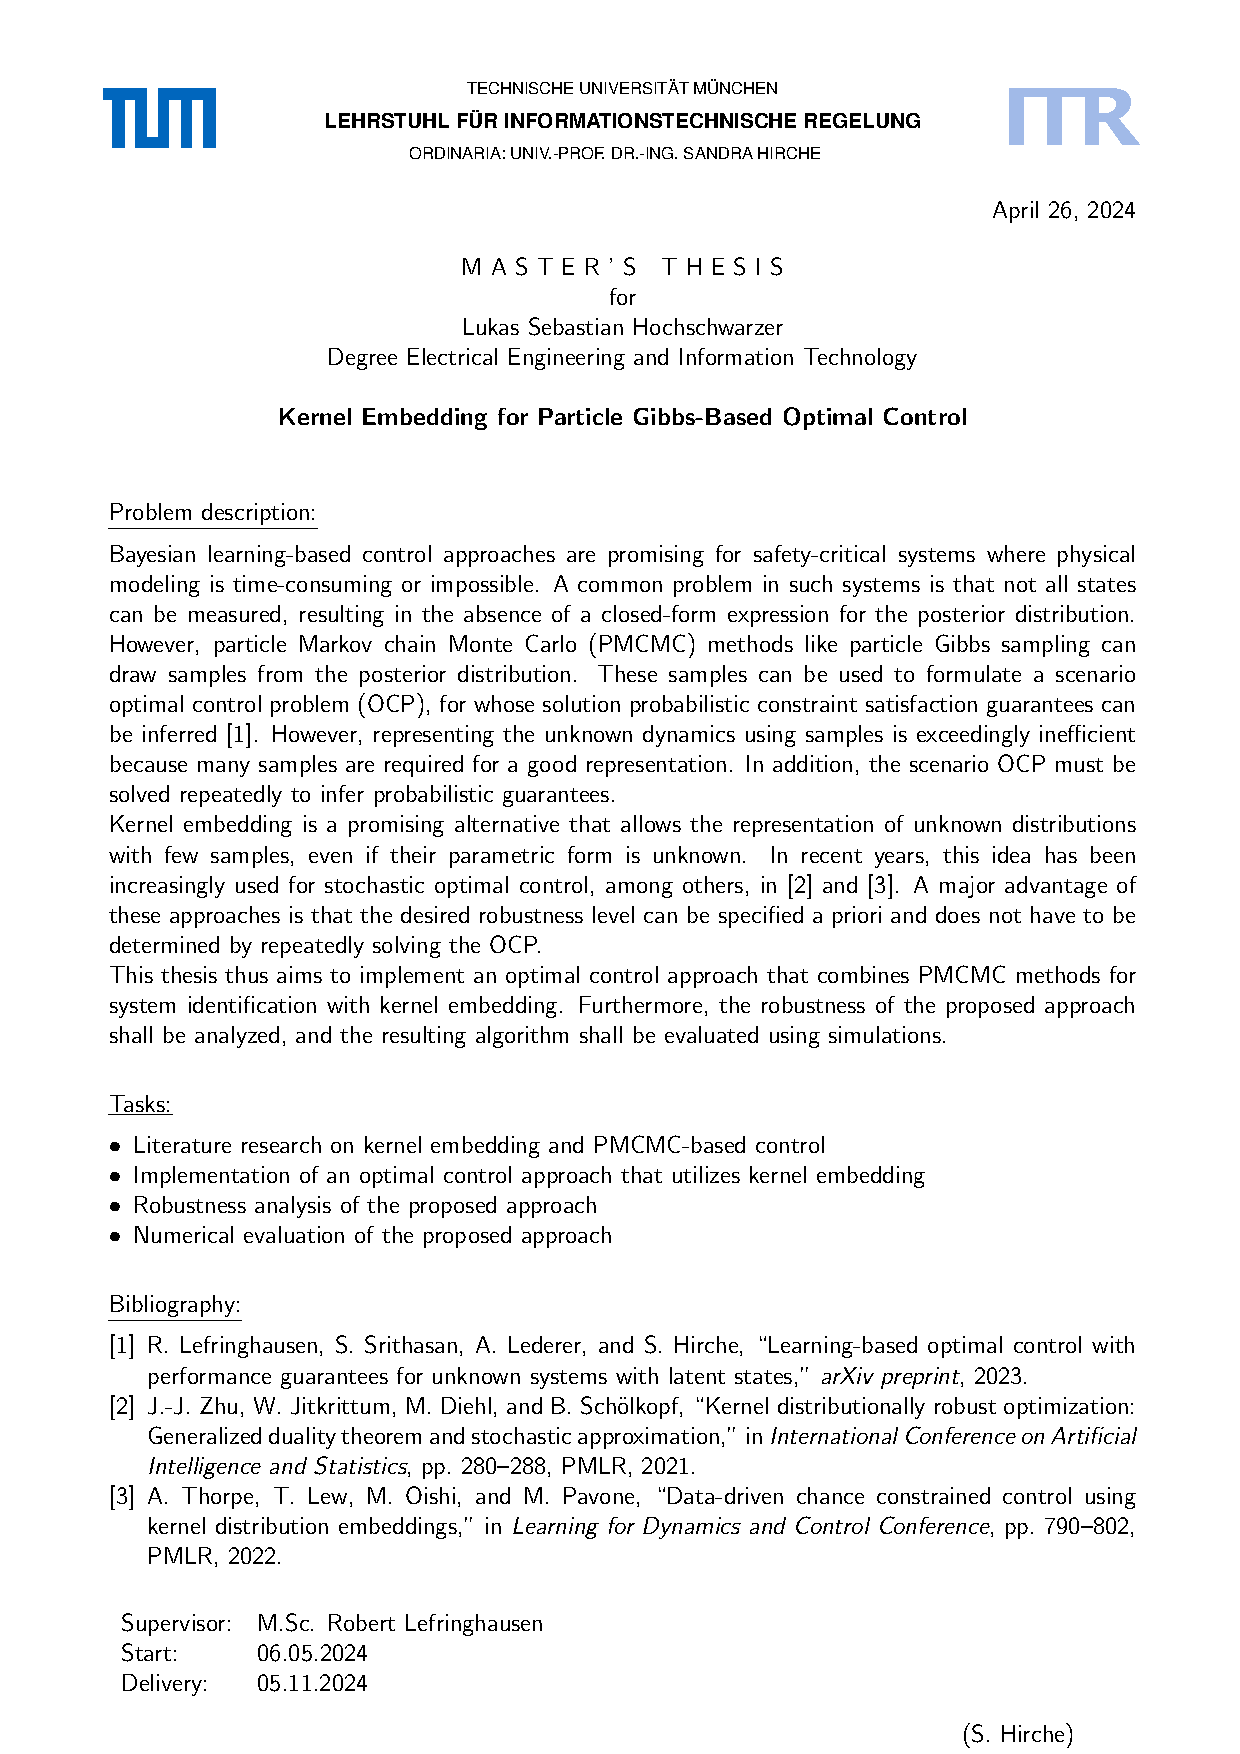
\includepdf[pages=1]{./include/task_desc.pdf}
\fi
\newpage

%%%%%%%%%%%%%%%%%%%%%%%%%%%%%%%%%%%%%%%%%%%%%%%%%%%%%%%%%%%%%%%
%%%%%%%%%%%%%%%%%%%%% Abstract %%%%%%%%%%%%%%%%%%%%%%%%%%%%%%%%
%%%%%%%%%%%%%%%%%%%%%%%%%%%%%%%%%%%%%%%%%%%%%%%%%%%%%%%%%%%%%%%
\topmargin5mm
\textheight220mm
\pagenumbering{arabic}
\phantom{u}
\begin{abstract}
  A short (1--3 paragraphs) summary of the work. Should state the problem, major assumptions, basic idea of solution, results. Avoid non--standard terms and acronyms. The abstract must be able to be read completely on its own, detached from any other work (e.g., in collections of paper abstracts). Do not use references in an abstract.

%% German abstract (optional)
%\begin{center}	
%\normalsize \textbf{Zusammenfassung}\\
%\end{center}
%% Add the German abstract here
\end{abstract}
\newpage

%%%%%%%%%%%%%%%%%%%%%%%%%%%%%%%%%%%%%%%%%%%%%%%%%%%%%%%%%%%%%%%
%%%%%%%%%%%%%%%%% Preamble / Acknowledgments %%%%%%%%%%%%%%%%%%
%%%%%%%%%%%%%%%%%%%%%%%%%%%%%%%%%%%%%%%%%%%%%%%%%%%%%%%%%%%%%%%
\phantom{u}
\phantom{1}\vspace{6cm}
\begin{center}
%% Insert preamble or acknowledgments here or leave blank
\end{center}

\pagestyle{fancy}

%%%%%%%%%%%%%%%%%%%%%%%%%%%%%%%%%%%%%%%%%%%%%%%%%%%%%%%%%%%%%%%
%%%%%%%%%%%%%%%%%%% Table of Contents %%%%%%%%%%%%%%%%%%%%%%%%%
%%%%%%%%%%%%%%%%%%%%%%%%%%%%%%%%%%%%%%%%%%%%%%%%%%%%%%%%%%%%%%%
\tableofcontents 

%%%%%%%%%%%%%%%%%%%%%%%%%%%%%%%%%%%%%%%%%%%%%%%%%%%%%%%%%%%%%%%
%%%%%%%%%% Actual Content of the Report / Thesis %%%%%%%%%%%%%%
%%%%%%%%%%%%%%%%%%%%%%%%%%%%%%%%%%%%%%%%%%%%%%%%%%%%%%%%%%%%%%%
\ifLSRITRtutorial
	%_________Template Tutorial__________________________________

\chapter{Working with this Template}
\label{sec:Tutorial}

Please carefully read the following instructions about student reports and specifically this template. The contents of Chap.~\ref{sec:Tutorial} summarize the basics about working with this template. The subsequent chapters focus on specific parts of your report, e.g., the introduction (Chap.~\ref{sec:introduction}).

\section{General Remarks}

\optional{Please have a look at our \href{https://wiki.tum.de/display/lsritr/Students}{\underline{thesis-guidelines}} before submitting your \emph{final} thesis.}

\subsection{Revisions of your thesis}

Hand in your thesis at minimum \textbf{one week} before the deadline for correction. You will receive feedback for the final version and very likely have to do minor or major revisions of your writing. Plan your writing schedule to allow for these adjustments, which can have quite some impact on your grade! 



\subsection{Structure of your thesis}

Make sure your thesis is well structured, that each major section does what it is supposed to do, and that the overall story is clear. This template offers a common basic structure (but other structures are possible). In particular, you do not need to have exactly as many major sections or chapters as the template implies; sometimes it makes sense to merge parts, sometimes it makes sense to move parts (e.g., the location of the literature review may vary), sometimes it makes sense to split a logical part into several individual sections. Just use some common sense. 

You do not have to write down everything you do. Focus on the main results of your work and structure your report accordingly. The goal is a structured report that provides everything needed to understand and replicate your work (data, formulas, parameter values, $\ldots$). Not everything that you do/read/plot during your work has potential to be put in the report. A longer report is not necessarily better!

A sample structure is briefly provided in the following. Note again that your report does not necessarily have to follow this sample structure perfectly.

\vspace{\baselineskip}


(Sample) Structure in a nutshell:

\begin{itemize}
	\item Chapter 1: Introduction
	\begin{itemize}
			\item General motivation - understandable even to your grandma.
			\item What has been done before? (related work: How do other people solve your problem? What are drawbacks of their approaches?)
			\item How do you approach the issue? What are the challenges? What methods do you use? What is new about your approach?
			\item Describe the structure of your report: 
			\item This report is structured as follows: Chap. 2 introduces $\ldots$ . In Chap. 3 $\ldots$ . $\ldots$ is discussed in Chap. 4. $\ldots$ and so on $\ldots$
			\item Optional: put notation here.
	\end{itemize}
	\item Chapter 2: Relevant methods - describe the methods and structures you use
	\item Chapter 3: Describe your approaches
	\item Chapter 4: Simulation results
	\begin{itemize}
			\item Describe the setup/model/implementation.
			\item Give all parameters necessary to replicate your results.
			\item Show results.
			\item Discuss results thoroughly (a critical view point is important here).		
	\end{itemize}
	\item Chapter 5: Experimental results (structure similar to simulation results)
	\item Chapter 6: Conclusion
	\begin{itemize}
			\item Summarize the goal of your work.
			\item Summarize your approach and your results.
			\item Draw conclusions.
			\item Give an outlook on possible future work.
	\end{itemize}
\end{itemize}

\newpage

\section{Structuring: Sections}

Use chapters, sections, and subsections to structure your document. 

\subsection{Subsection}

This is a subsection. 

\subsubsection{Subsubsection}

Subsubsections can be used to further structure information within a subsection. They do not show up in your list of contents. Please do not use more than these two ``sub''-prefixes to sections (no: subsubsubsubsection). If you feel that you need even finer grained structuring, rethink your overall structure.

\paragraph{Paragraphs} are sometimes more useful than subsubsections to structure text without breaking the flow.


\section{Style and Expressions}

Before handing in your thesis, even for an intermediate review, please perform a spellcheck and correct grammar mistakes. Proof-read your work thoroughly BEFORE you send it to your supervisor. Text/latex editors usually have a spell check option included - use it! Be aware that latex editors often do not have the most sophisticated spellchecks.

The report is not meant to be a narrative text. Please stick to neutral and technical style and avoid subjective or biased expressions or adjectives/adverbs such as \emph{obviously, always, very, especially well, actually, so-called etc}. Scientific writing is about precision and you should underpin your statements factually, not soften them with unnecessary qualifiers. Look at the papers you read and use them as a reference on how other people write scientifically.

If you know that you often make the same errors without meaning to (e.g., use past tense, forget protected spaces, use present progressive, use a word in the wrong way, $\ldots$) in many cases the search (or replace) function helps in finding them all.

\subsection{Writing}

Choose whether you want to write American English or British English and stick with it (more common is American English). If your spellcheck allows to set dictionaries, pick the appropriate language pack (British/US) to get corrections hints that help you to consistently write in either of the two languages.
Make sure you are aware of the basic rules of English grammar (sentence structure, adverbs with ``-ly'' at the end, use of punctuation, etc.).

Keep it simple: 

\begin{itemize}
	\item Simple and short sentences (subject - verb - object)
	\item Simple words you know even if it sounds repetitive (Your teacher probably told you in school, that you should find synonyms whenever possible. You can do this when you write in your native language and you have a feeling for the words. Otherwise it is okay to sound repetitive, especially for nouns. And in any case: Do NOT just use new words without thoroughly researching all their meanings, really, don't!)
	\item If you really cannot avoid using new words, double-check whether the word really means what you want to express (translate the word back into your mother tongue and check its other meanings)
\end{itemize}

Do not use ``I'', use ``we'' instead, but do not overuse as this may sound too casual for your report. Instead use a passive form or activated objects (e.g. ``The figure shows ...'', ``The robot moves ...''). Use present tense without exceptions (especially no past tense - NEVER - not even when you write about related work or in the conclusion). Instead use simple present (``We write this in our report.'') - never present progressive (``-ing'' forms: ``We are not writing this in our report.''). Also keep in mind that punctuation is not optional. Line breaks, on the other hand, should only be used whenever a new train of thought starts. Do not overuse them. Articles (the/a/an) are also NOT optional. If you are not sure which preposition (in, on, to, $\ldots$) to use with a word, remember: Some words are used with various prepositions, but then they often have different meanings! Do not overuse ``can'' or ``cannot''. There are other formulations that often fit better.

\section{References}

Use references to your equations/theorems/figures/etc. to make it easier for the reader to follow, especially when you need it again later in a different context.
References to chapters/sections/subsections are labeled with \verb|\label{...}| and referred to with \verb|\ref{...}|. Use: 

\begin{itemize}
	\item Capital ``Chapter\verb|~\ref{...}|'' for chapters or ``Section\verb|~\ref{...}|'' for sections and subsections with protected space ``\verb|~|'' at the beginning of sentences:
	\begin{itemize}
		\item Chapter 1/Section 1.1 describes $\ldots$ .
	\end{itemize}
	\item Capital ``Chap.\verb|~\ref{...}|'' for chapters or ``Sec.\verb|~\ref{...}|'' for sections and subsections with protected space ``\verb|~|'' within sentences:
	\begin{itemize}
		\item $\ldots$ is described in Chap. 1/Sec. 1.1.
	\end{itemize}
	\item Small ``chapter'' or ``section'' (NEVER subsection, $\ldots$ - these are also sections) if it is not followed by a reference:
	\begin{itemize}
		\item In the following chapter/section, the method $\ldots$ .
	\end{itemize}
\end{itemize}

\subsection{Equations}
Refer to equations whenever it helps in understanding your text. This makes it easier for the reader to follow your train of thought:
\begin{itemize}
	\item NEVER refer to an equation before you introduce it. 
	\item Equation numbers should be put in brackets (1.1) - use\verb|~\eqref{}|, which does it automatically for you. Use the protected space ``\verb|~|'' to avoid lines starting with equation numbers.
	\item Do not start a sentence with an equation number.
	\item Do not write ``equation'' before putting the reference:
	\begin{itemize}
		\item Bad: Given Equation (1.1), it is possible to show $\ldots$ .
		\item Good: Given (1.1), it is possible to show $\ldots$ .
	\end{itemize}
\end{itemize}

\subsection{Figures}

References to figures should be included in the following way:
\begin{itemize}
	\item Capital ``Figure\verb|~\ref{fig}|'' with protected space ``\verb|~|'' at the beginning of sentences:
	\begin{itemize}
		\item Figure 1.1 shows the motion of the point mass.
	\end{itemize}
	\item Capital ``Fig.\verb|~\ref{fig}|'' with protected space ``\verb|~|'' within sentences:
	\begin{itemize}
		\item The motion of the point mass is shown in Fig. 1.1.
	\end{itemize}
	\item Small ``figure'' if it is not followed by a reference:
	\begin{itemize}
		\item The figure also shows $\ldots$ .
	\end{itemize}
\end{itemize}

\subsection{Tables}

Tables make it easy to understand the content. Less lines are sometimes better and look nicer, take a look in literature.
References to tables should be included in the following way:
\begin{itemize}
	\item Capital ``Table\verb|~\ref{tab}|'' with protected space ``\verb|~|''  at the beginning of sentences:
	\begin{itemize}
		\item Table 1.1 lists $\ldots$ .
	\end{itemize}
	\item Capital ``Tab.\verb|~\ref{tab}|'' with protected space ``\verb|~|''  within sentences:
	\begin{itemize}
		\item $\ldots$ are given in Tab. 1.1.
	\end{itemize}
	\item Small ``table'' if it is not followed by a reference:
	\begin{itemize}
		\item The table also lists $\ldots$ .
	\end{itemize}
\end{itemize}	

\subsection{Definitions / Assumptions / Theorems / Lemmas}

Basically, the same applies as for figures, tables, chapters, and sections:
\begin{itemize}
	\item Use protected spaces ``text\verb|~\ref{...}|''.
	\item Capital and full word (Definition/Assumption/Theorem/Lemma/Proposition\verb|~\ref{}|) at the beginning of sentences.
	\item Capital and short form (Def./Ass./Th./Lem./Prop.\verb|~\ref{}|) in the middle or at the end of sentences.
	\item Small and full word (definition/assumption/theorem/lemma/proposition) if used without reference.
\end{itemize}

\section{Equations}
Include equations in your text in a meaningful way. Example: 

\vspace{\baselineskip}
\fbox{\parbox[c]{\textwidth}{

The equation of motion of a point mass is given by 
\begin{equation} m \ddot{x} = f \ , \label{eq:motion} \end{equation}

where~$m\in\mathbb{R}$ is the mass,~$f\in\mathbb{R}$ the externally applied force, and~$\ddot{x}\in\mathbb{R}$ the acceleration in~$x$-direction.}}

\vspace{\baselineskip}

You can use~\eqref{eq:motion} to reference an equation in the
text. Equations without reference number:
\[
y=x^2
\]



Please type all numbers in mathematics mode.
Mathematical equations that are not part of the text should be centered. If you have multiple lines with equations, align equations with the arithmetic operator \verb|(=,<, ...)|:
\begin{subequations}
\begin{align}
a &= 2\\
b&= 3+4
\end{align}
\end{subequations}
Type physical units as normal text, e.g., s, not $s$! (the package \textit{siunitx} helps)
Formulas must not jut out over the text margin, so take care to stay within the margins and eventually break the equation into several lines.
Explain the variables you use. For each newly introduced variable, at least a short description of the variable should follow the equation in the style of \emph{\ldots with $x$ being the position of the cart and $u$ the control input.} Use variable names whenever possible to make it easier for the reader to make the connection: 
\begin{itemize}
\item[-] Bad: A high mass slows down the acceleration. 
\item[-] Good: A high mass~$m$ slows down the acceleration.
\end{itemize}
A parameter or variable must not be used at the beginning of a sentence.
Mathematical units must be consistently labelled with only one variable. \hl{Do not
use a variable for more than one mathematical unit}.

If you use in-line equations, either to introduce parameters or for actual equations, put a ``\verb|~|'' in between the in-line equation and the preceding word. This is a protected space - it avoids that the equation is moved to the next line, which would be considered bad style. 

If you use descriptive text in equations, set it as \verb|\text{}|. Examples:
\begin{itemize}
	\item $x_{\text{measured}}$: ``measured'' is descriptive here and not a variable/parameter 
	\item $q_{\text{des},i}$: ``des'' is descriptive here but ``$i$'' is a counter and therefore not in text 
\end{itemize}

If you want to generate more sophisticated equations, use the \textit{IEEEtrantools} package. 
%, which is used as follows:
%\begin{IEEEeqnarray}{r c l}
%\IEEEyesnumber
%a =& b &= c \IEEEyessubnumber \\
%c =& d+e &= 5 \IEEEyessubnumber
%\end{IEEEeqnarray}
This package is especially useful if custom spacing is required for multiple equation lines.

\subsection{Notation Consistency}

Consistency is key: Choose a style for your notation and stick with it. We suggest giving a notation list somewhere in your report (ideally in the beginning). 
Most often used:
\begin{itemize}
	\item vectors: bold, small letters \verb|\mathbf{}| ($\mathbf{a}$) or \verb|\boldsymbol{}| ($\boldsymbol{a}$)
	\item matrices: bold, capital letters \verb|\mathbf{}| ($\mathbf{A}$) or \verb|\boldsymbol{}| ($\boldsymbol{A}$)
	\item scalars: small (sometimes also capital), non-bold letters ($a$)
	\item general sets: \verb|\mathcal{}|
	\item sets of numbers (real, whole, $\ldots$): \verb|\mathbb{}| ($\mathbb{A}$)
\end{itemize}

\subsection{Symbol Glossary}

Instead of writing mathematical symbols individually in each equation, you can also use a glossary entry. For example, instead of explicitely writing \verb|\mathbf{u}_k| to denote a control input $\mathbf{u}_k$ at time step $k$, you can define a glossary entry, e.g., ``uk'', and just use \verb|\gls{uk}|, which then also yields \gls{uk}. Glossary entries for symbols are defined in the file ./include/gloss.tex.

This procedure is useful for two reasons: 1) You can shorten long symbol expressions significantly. 2) If you later want to change a symbol, you only need to change the glossary entry once - you don't need to change every single symbol in your document.

\subsection{Style Notes}

There are a few important style notes to consider in equations.
\begin{itemize}
\item Indices: Use italic font for math-related indices (parameters, variables, ...) and non-italic font for other descriptions, e.g., $x_t$ (time $t$) and $x_{\text{ref}}$ (ref: reference).
\item Mathematics operations are non-italic, e.g., $\sin(x)$. Often, functions are already defined in latex (e.g., use \verb|\sin(x)|). If not, use \verb|\mathrm{}|, e.g., $\mathrm{sin}(x)$.
\item Make sure parentheses are large enough by using \verb|\left( . \right)|, e.g., \[\left( \frac{1}{2} \right) \textnormal{instead of } ( \frac{1}{2} ) .\]
\item Use \verb|^\top| for a transpose, e.g., $\boldsymbol{x}^\top$.
\end{itemize}



\section{Figures}

For pictures, you can use .pdf, .jpg, .png, etc when working with \textbf{pdflatex}; with \textbf{latex} you need .eps:
\begin{figure}[htb]
\centering
%\includegraphics[width=0.2\textwidth]{lsr_logo}
%\includegraphics[width=0.9\textwidth]{abbildung.eps}
\caption[Abbreviated Description]{Long Description: The subtitles of tables and illustrations should be self-explanatory.}
\label{fig:abb1}
\end{figure}

Figures should be vector graphics (pdf or eps) and self-made (to avoid blurry pictures). We recommend pgfplots/tikzpiktures or inkscape and Matlab (export figure with tick set at Rendering - Custom renderer: painters) in combination with \verb|\psfrag{ }[ ][ ]{ }| to replace the text in \LaTeX.

Every illustration must be described and referenced in the text, cf. Fig. \ref{fig:abb1}. 
There is no such thing as a decorative figure! 
If the figure is not mentioned in the text and therefore lacks an explanatory function, leave it.
Lines in plots need to be clearly distinguishable, also in black-and-white print. Therefore, choose your colors and line styles wisely and consistently!
The subtitles and axis labels must be clearly legible (i.e., big enough) and include a scaling. Ideally, the figure is self-explanatory with labels, arrows, text, etc. Text in figures should be without serif: \verb|{\sf your_text_goes_here}|, about the same size as the ``normal'' text and labels should include all important information such as the name of the depicted variable and the corresponding unit. Captions should clearly describe the content. If the caption is rather long, use ``\verb|\caption[short_caption]{long caption}|''. The long caption appears below the figure, the short caption appears in the list of figures. 

Figure axes need to be labeled correctly. Do not just mention the variable name but include a description. If units are required, use parenthesis. An example is given in Fig.~\ref{fig:vel_plot}.

\begin{figure}[htb]
\centering
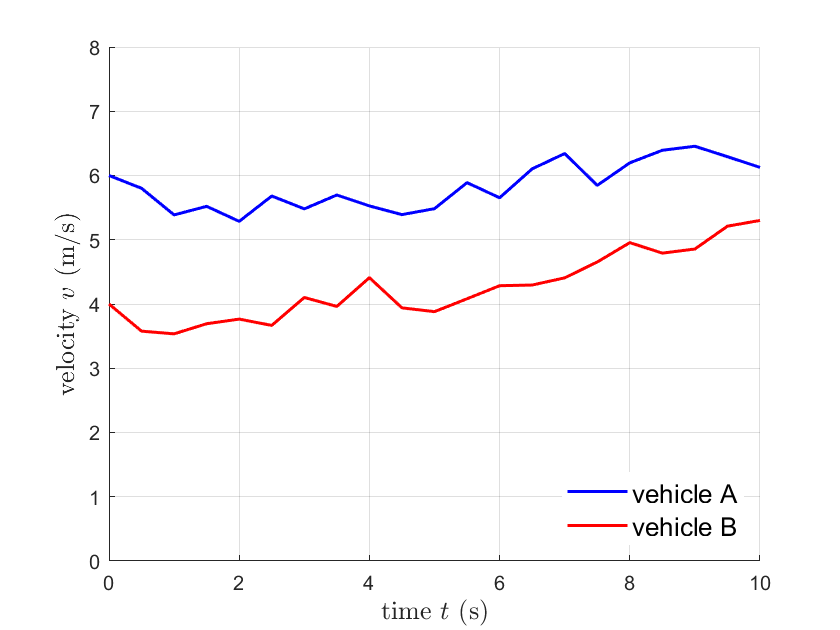
\includegraphics[width=0.6\textwidth]{pics/velocity_plot.png}
\caption{Example velocity plot with units}
\label{fig:vel_plot}
\end{figure}

If the illustration is copied from another person's work, you need to mention the
source with \verb|\cite{}|.

By using \textit{subfigure}, several pictures can be combined in one main picture as in Fig.~\ref{fig:OverallPic}:

\begin{figure}[htb]
\centering
\subfigure[Subfigure 1 caption]{
   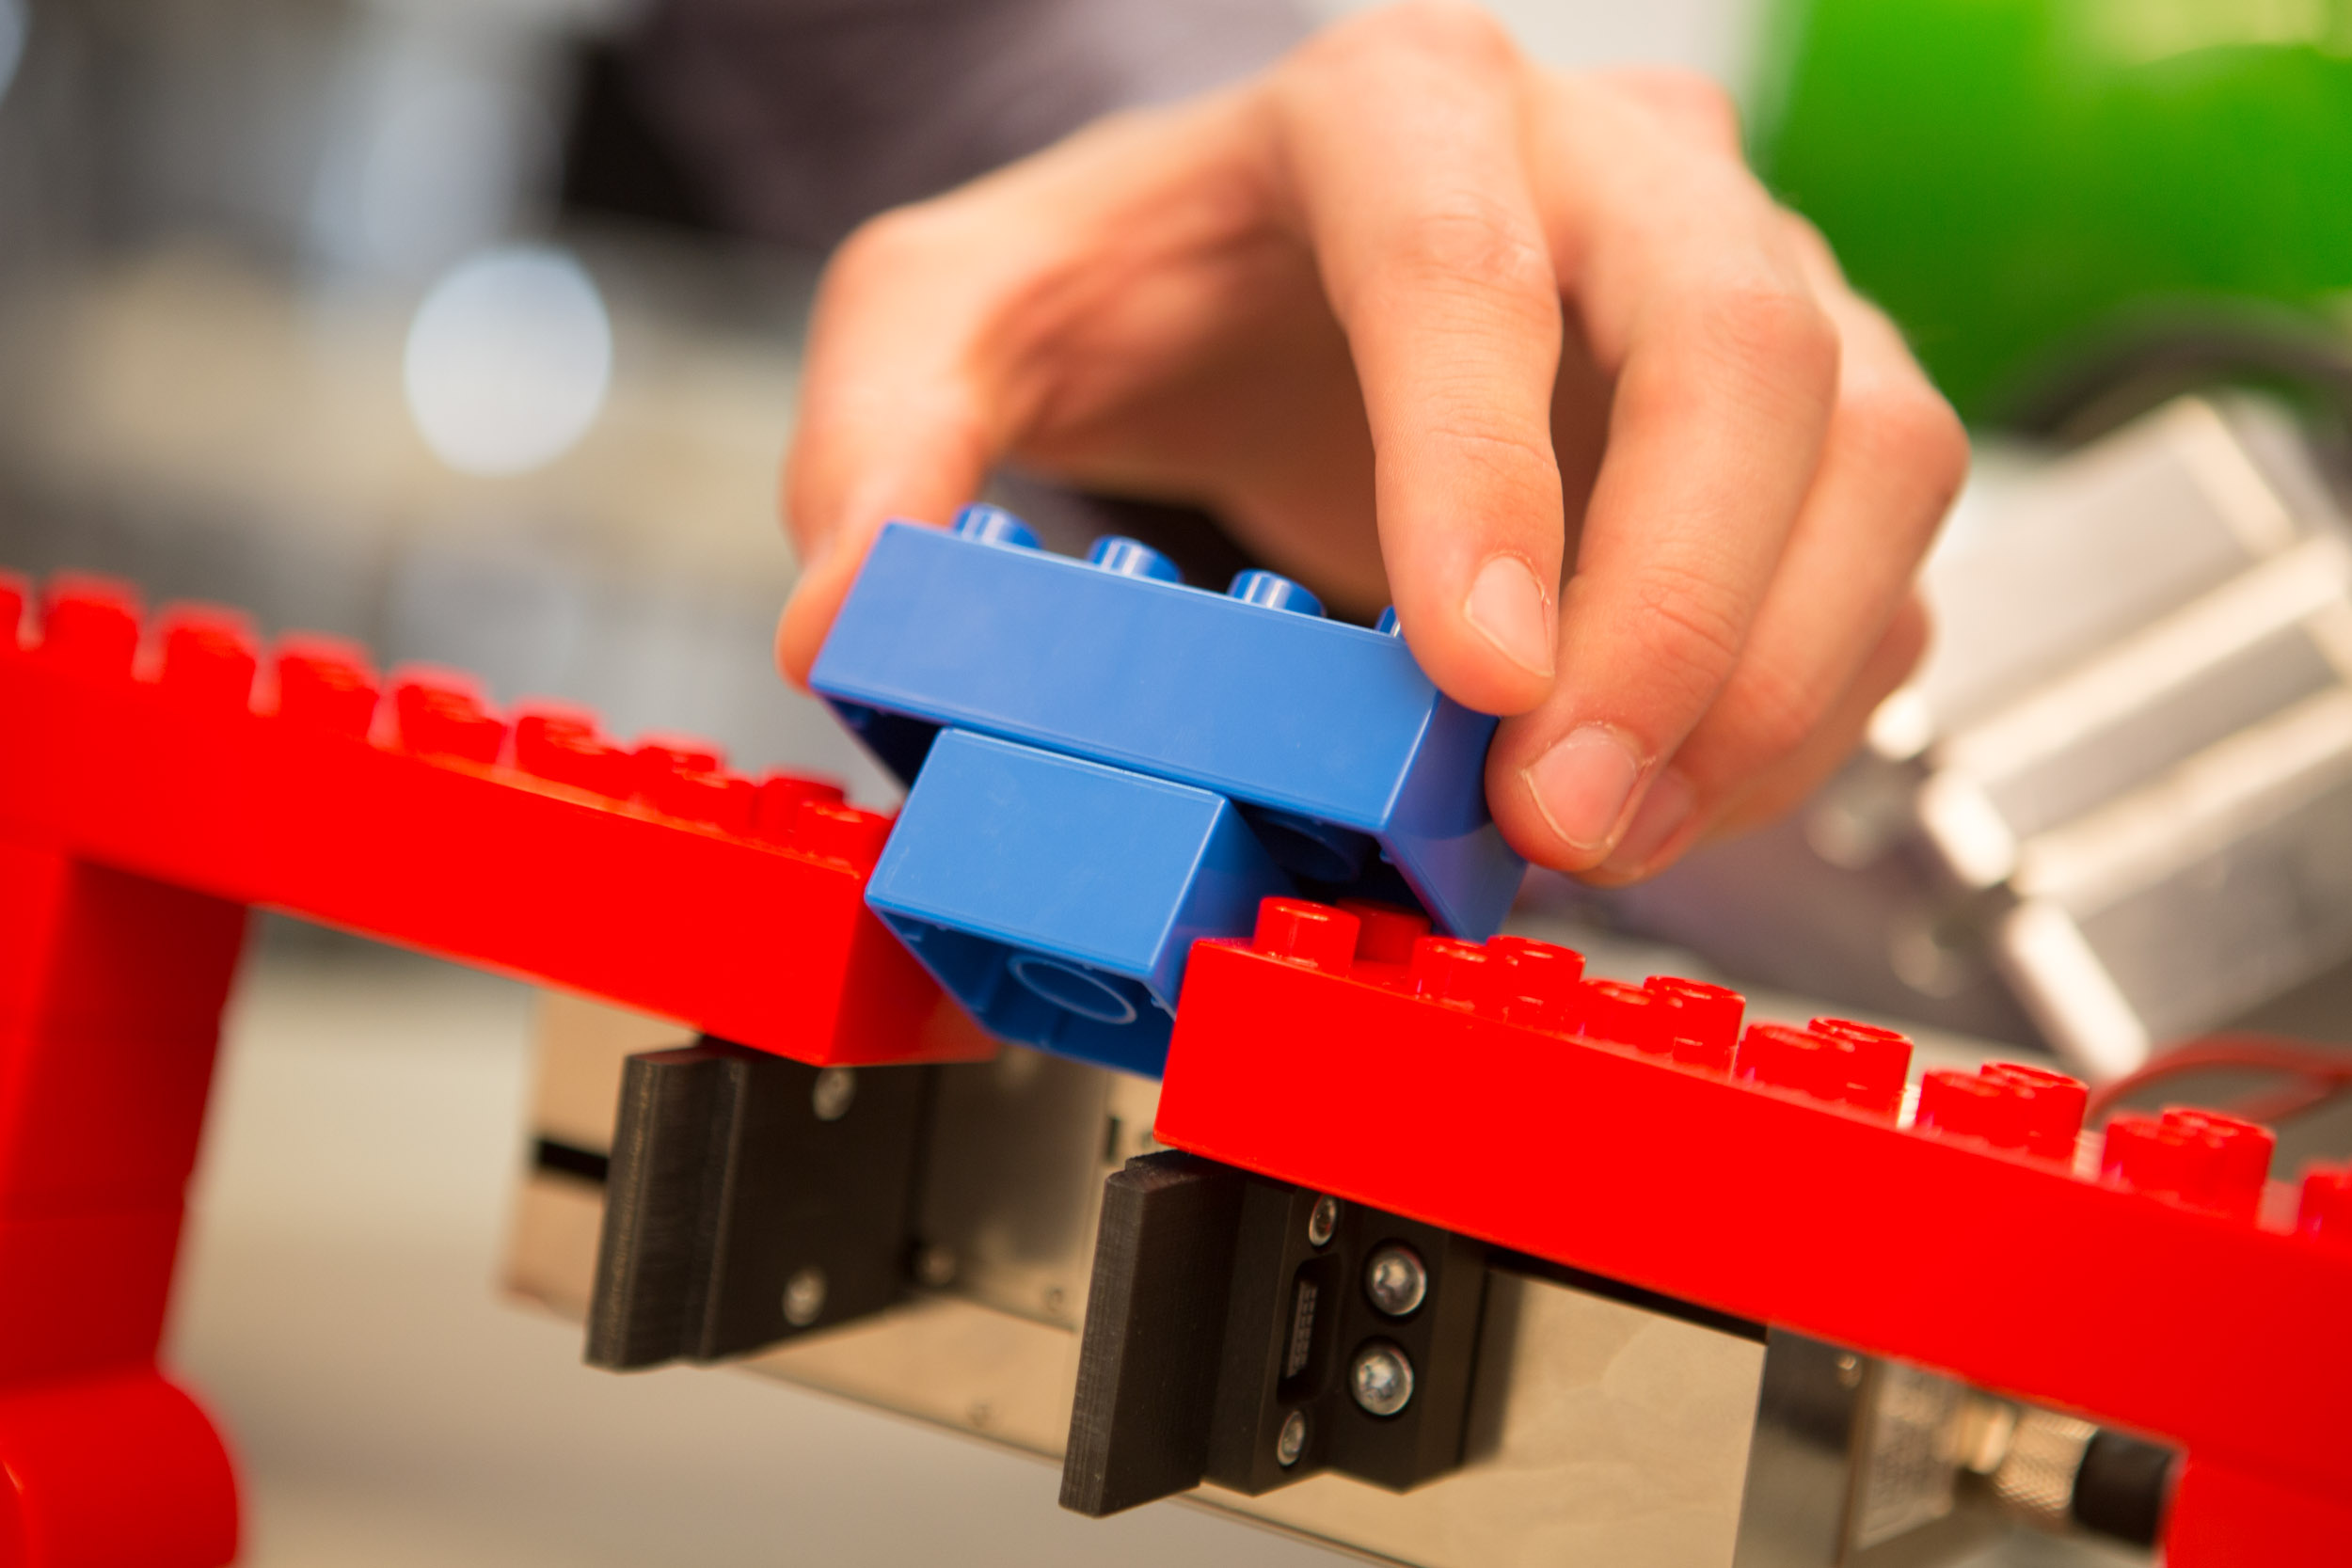
\includegraphics[width=0.3\textwidth] {Lego_robot3}
   \label{fig:subfig1}
 }
\quad % puts next subfigure right next to the previous subfigure
\subfigure[Subfigure 2 caption]{
   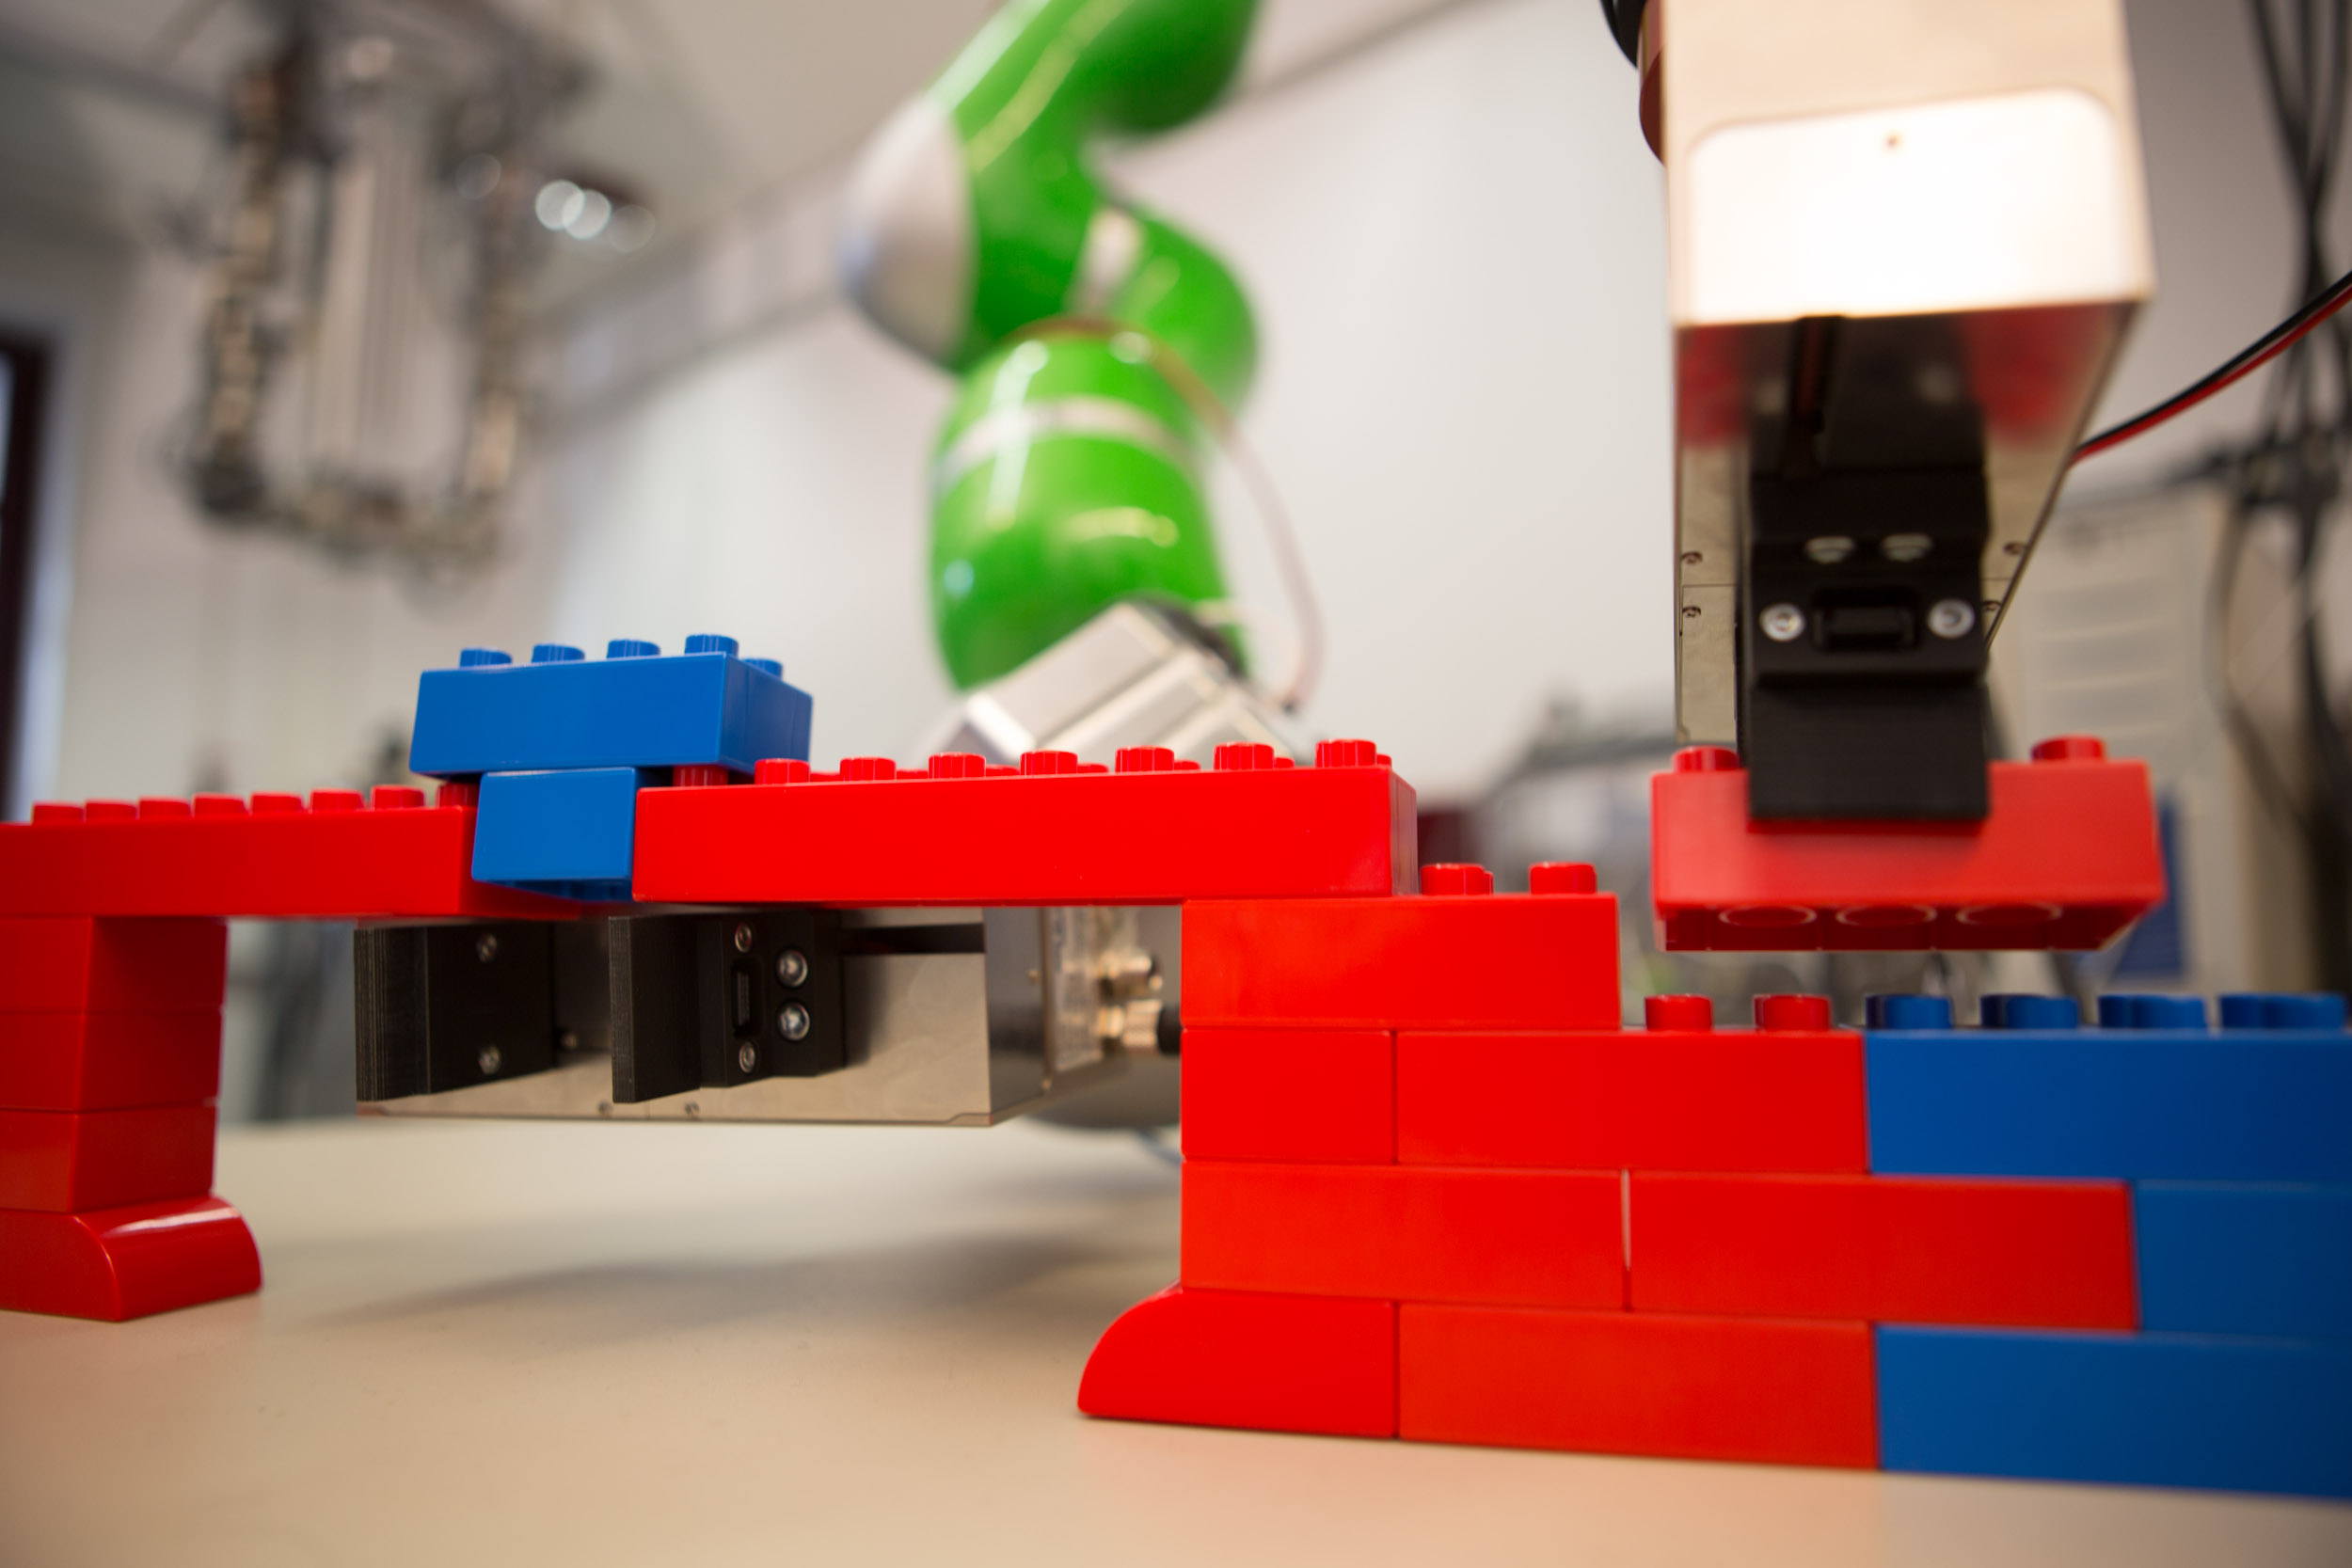
\includegraphics[width=0.3\textwidth] {robot_build}
   \label{fig:subfig2}
 }

\subfigure[Subfigure 3 caption]{
   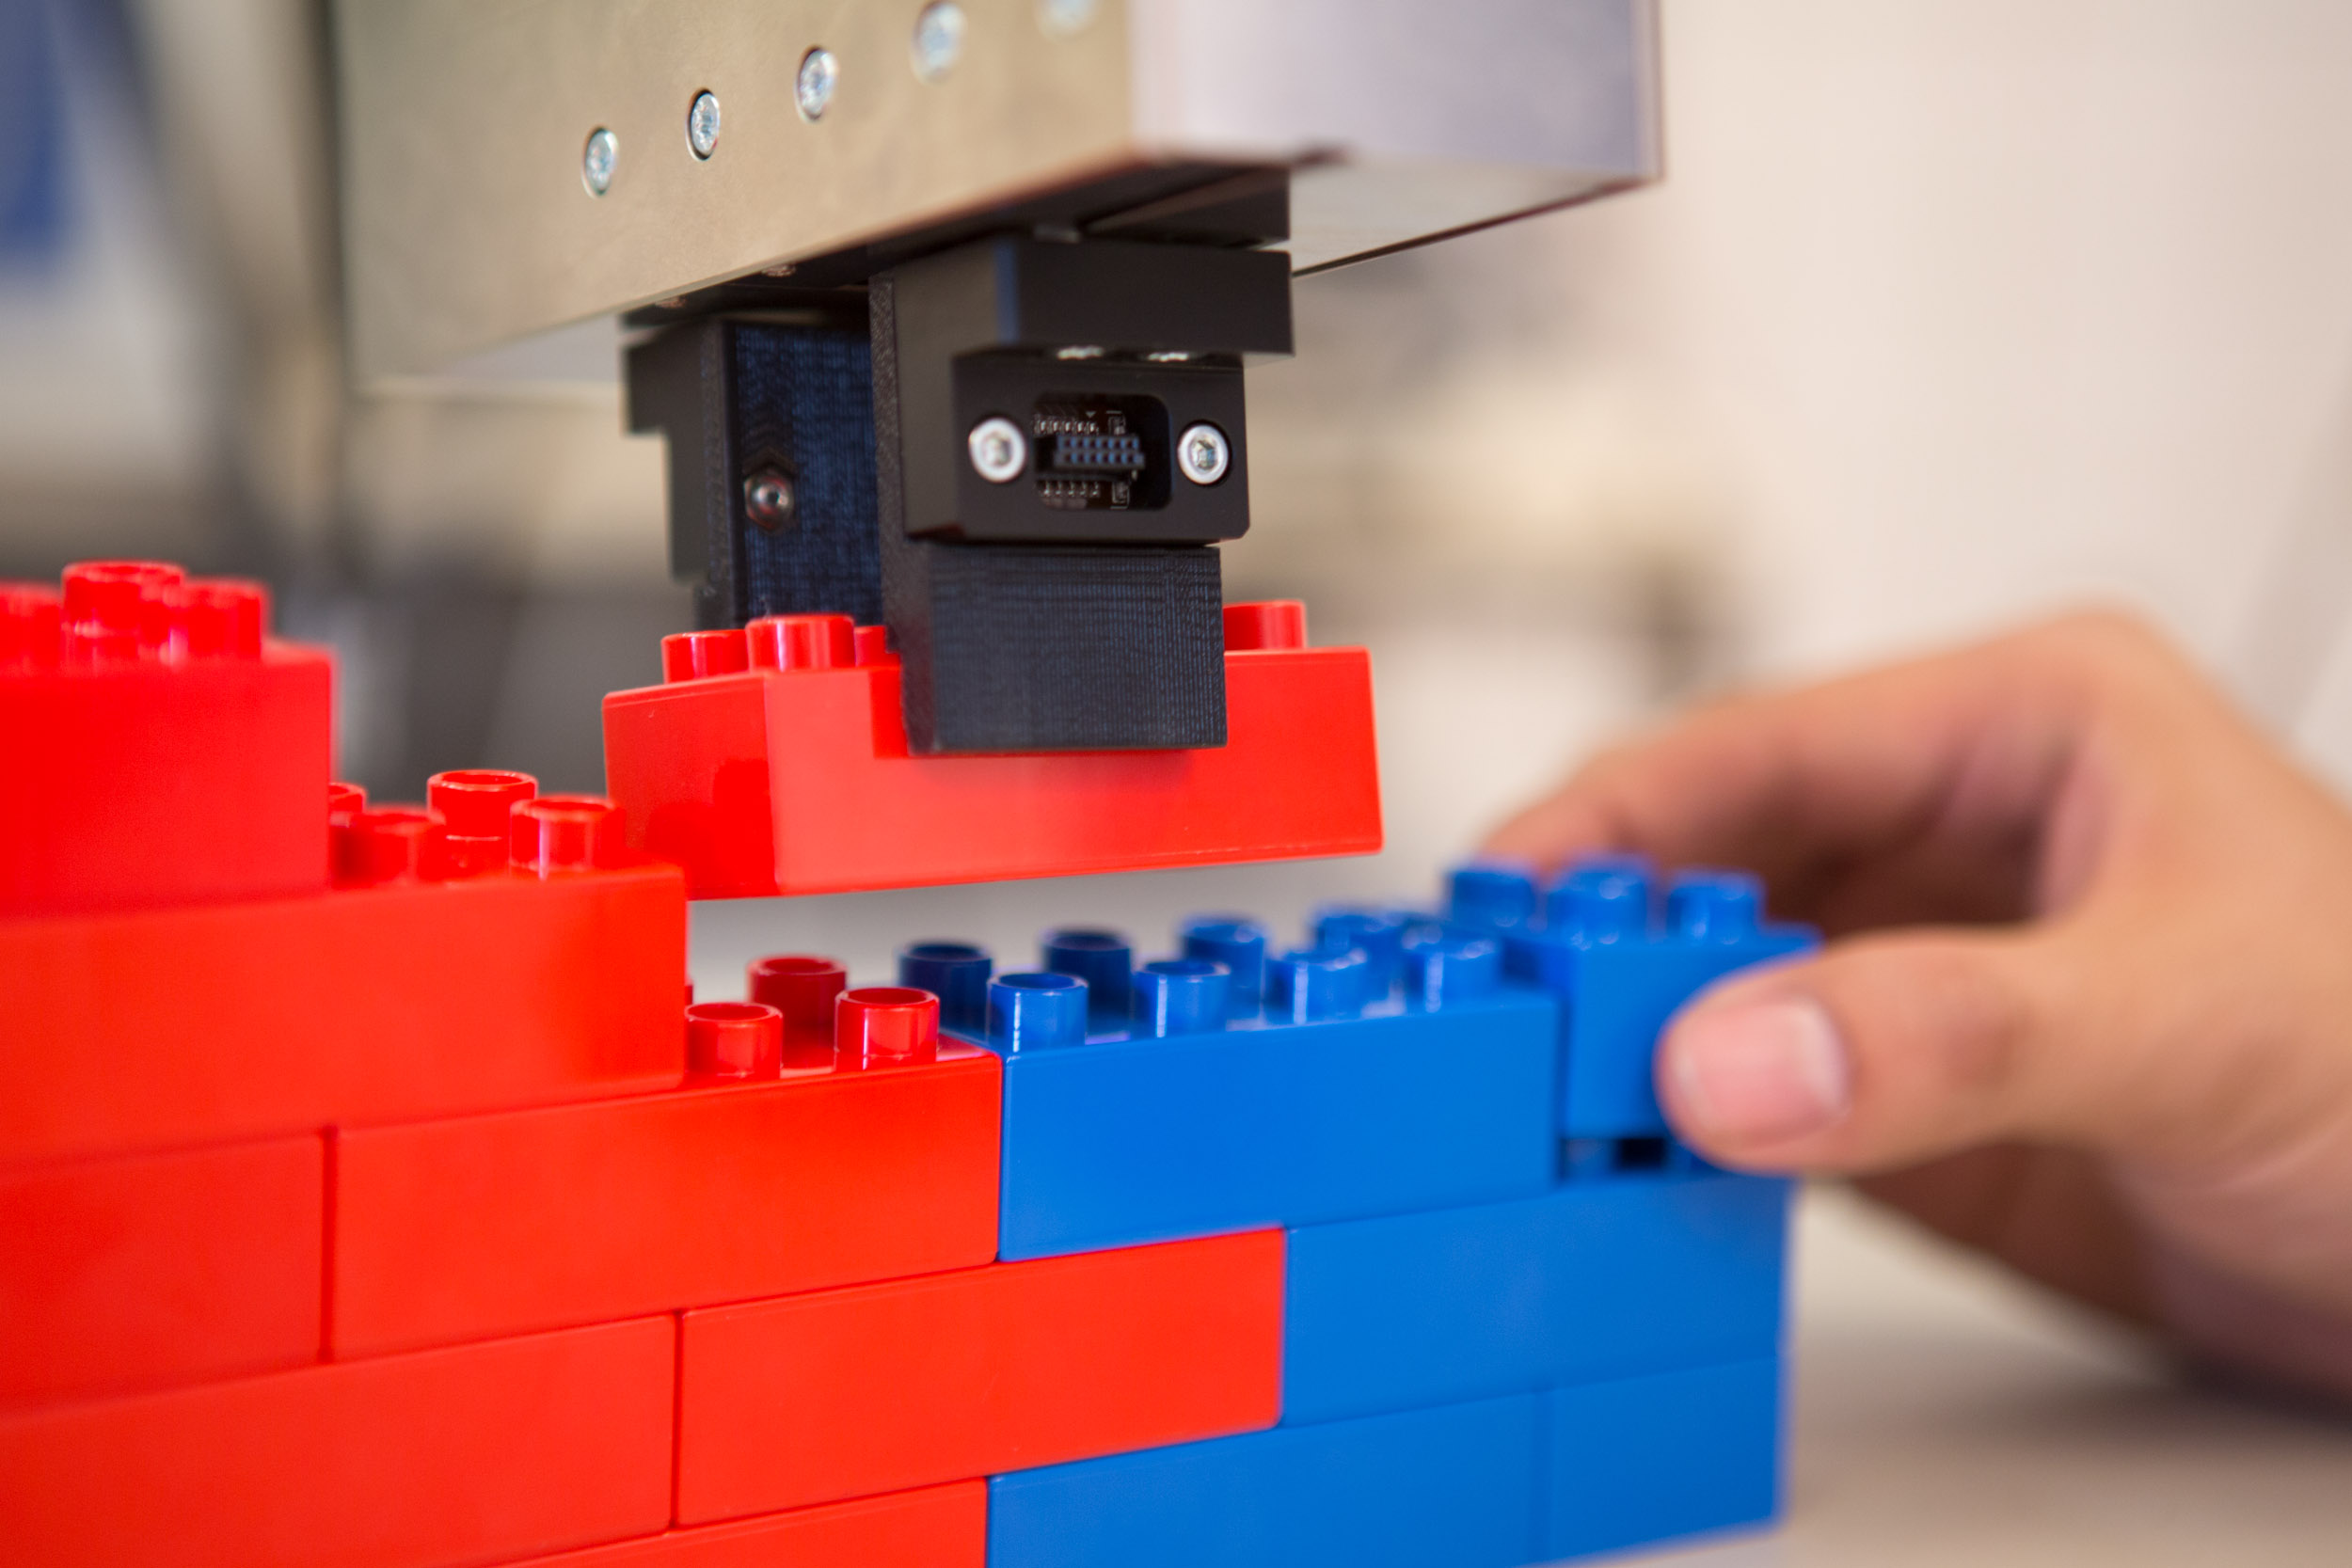
\includegraphics[width=0.4\textwidth] {robot_build_withHuman}
   \label{fig:subfig3}
}
\subfigure[Space-holder for missing picture]{
	\missingfigure[figwidth=0.4\textwidth]{
		\tiny{A Picture needs to be  put here later. One can use acronyms, e.g. \gls{HRC}}}
	\label{fig:subfig4}
}  
\caption[Abbrev. Descr. of subfigure-figure]{A figure with two subfigures}
\label{fig:OverallPic}
\end{figure}

This figures can be referenced by either referencing the overall label \ref{fig:OverallPic} or a specific subfigure label \ref{fig:subfig1} - if the labels have been set properly of course! The subfigures are not listed in the list of figures!



\section{Definitions / Assumptions / Theorems / Lemmas}

Sometimes a definition is helpful, especially for later reference. Motivate and introduce each one and do not just list definitions one after another. Explain why it is important and what it is used for. Assumptions are useful to emphasize what preliminaries have to be fulfilled for your approach to work, especially if you plan to introduce theorems, lemmas, etc. 

Points to remember:
\begin{itemize}
	\item Do not list assumptions one after another. 
	\item Motivate and introduce each one.
	\item Explain how restrictive it is and illustrate its effects on the application.
\end{itemize}

Sometimes you need to cite a theorem/lemma/proposition. 

Points to remember:
\begin{itemize}
	\item Same as above: do not just list, motivate, introduce, explain what this enables.
	\item Make yourself familiar with the way theorems/... are usually formulated. Look at the literature. 
	\item Make sure all relevant assumptions and preliminaries are stated in the theorem/...
	\item Make the proof (if it is your own theorem/...) conclusive and understandable.
\end{itemize}



\section{Citations}

Citations are extremely important and \textbf{must} be included whenever you use other people's work. Direct citations with directly copy-pasting the content and marking it with ``$\ldots$'' are unusual in scientific reports. Always try to reformulate the source into your own words to generate an indirect citation. 


Whether to use numeric or alphabetic references is not all that important (unless prescribed by a conference or journal), but alphabetic tends to be more readable. Independent of citation style, the following rules should be followed:

\begin{itemize}
\item Use the \LaTeX~cite package. It does not give you additional commands, but it fixes a few quirks in \LaTeX. Among others, it automatically sorts multiple citations, and it correctly spaces the angular brackets (if you use the \verb|\cite{}| command without leading white space).

\item Citing several papers at one point should be done with a single \verb|\cite{}| command. For example, use \verb|gives good results\cite{Bloe_99, Jay_87}|, resulting in gives good results \cite{Bloe_99, Jay_87}. 

Do not use \verb|gives good results\cite{Bloe_99}\cite{Jay_87}|, which produces the ugly gives good results \cite{Bloe_99}\cite{Jay_87}. Also, note that there is no space between the \verb|\cite{}| command and the preceding word, \LaTeX~(with the cite package) does the spacing correctly.

\item Avoid citations of the kind: \cite{Bloe_99} thinks that $x>y$ is valid, but \cite{ONeill_2000} argues that this is invalid in case of $z\geq5$. This works a bit better if using alphanumeric citation labels. Better, though, use the authors' names: Bloe and Joe [1] think that $x>y$ is valid, but O'Neill et al. \cite{ONeill_2000} argues that this is invalid in case of $z\geq5$. 

\item Avoid citations at the beginning of a sentence:
	\begin{itemize}
		\item Bad:
		\begin{itemize}
			\item \cite{Bloe_99} introduces different methods for motion control. (citation at the beginning)
			\item Different methods for motion control are introduced in literature. \cite{Bloe_99} (citation after the punctuation)
			\item Different methods for motion control are introduced in\cite{Bloe_99}. (preceding space missing or wrong cite package)
		\end{itemize}
		\item	Good: 	 
		\begin{itemize}
			\item Different methods for motion control are introduced in \cite{Bloe_99}.
			\item Khalil et al. introduce different methods for motion control \cite{Bloe_99}. 
			\item Motion control as in \cite{Bloe_99} is generally used to $\ldots$ .
			\item Motion control \cite{Bloe_99} is generally used to $\ldots$ .
			\item Motion control is generally used to $\ldots$ \cite{Bloe_99}.
		\end{itemize}
	\end{itemize}


\item BibTeX is a great tool, but you need to know how to use it. A regular trap is to forget that \TeX~knows more about typesetting than you do. So, for example, it changes the case of words in the title. If your title contains acronyms and proper names (most do), they tend to get down-cased. Any such words which should not have their case changed should be put into braces, e.g., \verb|{The {Mungi} {OS} and its Use in Merry-Go-Round Seat Allocation}|.


\item In citations do not abuse the category technical report. People tend to cite just about anything that has not been published in a journal or conferences as a TR. This is outright wrong. The concept of a TR is actually fairly well defined: A TR is published in some sort. This is generally as part of a formal TR series of some institution, in hardcopy or on the web or both. (They are not always called ``technical report'', other common names are ``research report'', ``technical memorandum'', $<$institution$>$ ``report'' etc.) The publication (i.e., availability outside) is essential, otherwise it's at best an internal report.
A TR has a number (absolutely!), an institution (publisher), a date (month and year at least) and a publisher's address (besides all the other stuff bibentries have).
If your document doesn't have these features, it's not a TR. It is probably better categorized as a working paper. Even then it has a date and an institution address.

\item Citing web pages is often unavoidable (but also often a sign of laziness). When citing web pages be aware that they may only be short-lived. Consider whether the reference will be of any use to the reader at all if the link is broken. Or whether your whole document only has a use-by date a few months past writing.

\end{itemize}

Any cited document, whatever it may be, has a few \textbf{mandatory} features:
\begin{itemize}
	\item Date. Absolutely. 
	\item Author/organization/creator/person responsible for contents.
	\item Whatever information the reader needs to find that document. In most BibTeX entry types these are clearly identified as mandatory fields. Mandatory means that they aren't optional. Do not pretend they are. For a working paper these might be the contact details of the author.
\end{itemize}


For bibliography, edit {\tt mybib.bib} and list all
references in a special style, e.g., for a book: 
\begin{verbatim}
@book{literaturstelle1,
 author    = {S. Sastry},
 title     = {Nonlinear Systems - Analysis, Stability, and Control},
 publisher = {Springer},
 year      = 1999
}
\end{verbatim}

Cite references in the text by \verb|\cite{citationreference}|.

In order to have your references shown in your PDF, compile by:

\begin{verbatim} 
latex myfile
bibtex myfile
latex myfile
latex  myfile
dvips myfile
ps2pdf -sPAPERSIZE=a4 myfile.ps
\end{verbatim}

Alternatively you can use your preferred \LaTeX -editor. The according BibTeX compiler has to be configured properly and then run before running PdfLaTeX. We recommend you to use our preconfigured editors.

\hl{Make sure your bibliography is consistent (e.g., all first names abbreviated).}

\section{Compiling}
Linux: 
do the following in a Shell:\\
\begin{verbatim}
latex myfile
dvips myfile
ps2pdf -sPAPERSIZE=a4 myfile.ps
\end{verbatim}
Make sure to use the A4 option, when you print the pdf!

Alternatively you can use either Kile, Texmaker, etc. on Linux or TeXnic Centre, etc. on Windows. Please be aware you have to set the required \LaTeX paths in your editors. The most common \LaTeX -editors in Linux are preconfigured at LSR and should work \emph{out-of-the-box}.





\fi
%_________Einleitung__________________________________
\chapter{Introduction}
\label{sec:introduction}

In the realm of model-based control, the development of reliable and accurate mathematical models is crucial to ensuring the success of any control application. However, finding such a model based on physical knowledge is often very time-consuming or even impossible. Because of this, data-driven control approaches that allow the derivation of such models based on previously collected data are gaining attention, and their usefulness for optimal control applications is being explored. For safety-critical applications, it is especially important to be able to account for uncertainties that result from basing the model on a limited set of training data (epistemic uncertainty) and the inherent randomness of the system, such as measurement noise (aleatory uncertainty). To this end, there are already numerous methods, such as a combination of state-space models and Gaussian processes \cite{Williams_06} or similar Bayesian approaches, that allow for reliable quantifications of uncertain models.

These approaches do, however, require full-state measurements of the unknown system in order to learn the model, quantify uncertainties, and make predictions, which is often not possible as these measurements are not available in numerous practical applications. In many applications, it is unknown which variables directly affect the system, or some states are not measurable. While methods such as NARX approaches \cite{Maiworm_21} exist that do not require the state space representation, they come with the disadvantage of it not being clear how to include the underlying physics of the model in the learning process. Having no knowledge of the states can also lead to these methods being unable to distinguish between the noise that permanently affects the system (process noise) and the noise that only affects one specific measurement (measurement noise). 

This means it is often advantageous to work with state-space models and, in the case of latent states, overcome the reliance on state measurements by jointly estimating the unknown dynamics and the latent states to create a reliable model for the system. This idea is already being utilized for optimal control in \cite{Robert_24} to estimate the uncertain elements of the system and use the acquired data combined with scenario theory \cite{Garatti_22} to obtain a robust solution. However, with this approach, the performance guarantees, i.e., a lower bound for the probability that the solution is feasible, have to be determined retroactively with a computationally complex process.
 
In this thesis, we propose how the use of kernel embeddings \cite{Yassine_22} as a way to reformulate the chance-constrained problem by using samples drawn from a distribution that is generally analytically intractable. This is possible by using particle Markov chain Monte Carlo (PMCMC) methods which allow us to jointly estimate dynamics and latent states. This enables us to include the allowed risk factor in the optimization process as a way to set performance guarantees in advance.

In this chapter, the problem is introduced in Section \ref{Problem Statement}, and related work is discussed in Section \ref{Related Work}. Finally, a quick overview of the structure of the rest of this thesis is given in Section \ref{Structure of this Thesis}.

\section{Problem Statement} \label{Problem Statement}

Consider the general nonlinear discrete-time system of the form

\begin{subequations} \label{System equation}
\begin{equation}
\boldsymbol{x}_{t+1} = \boldsymbol{f} \left( \boldsymbol{x}_{t}, \boldsymbol{u}_t \right) + \boldsymbol{v}_{t}
\end{equation}
\begin{equation}
\boldsymbol{y}_{t} = \boldsymbol{g} \left( \boldsymbol{x}_{t}, \boldsymbol{u}_t \right) + \boldsymbol{w}_{t}
\end{equation}
\end{subequations}

with the state $\boldsymbol{x}_t \in \mathbb{R}^{n_x \in \mathbb{N}}$, the input $\boldsymbol{u}_t \in \mathbb{R}^{n_u \in \mathbb{N}}$, the output $\boldsymbol{y}_t \in \mathbb{R}^{n_y \in \mathbb{N}}$, the process noise $\boldsymbol{v}_{t} \in \mathbb{R}^{n_x}$, the measurement noise $\boldsymbol{w}_{t} \in \mathbb{R}^{n_y}$ and time $t \in \mathbb{Z}$. 

In our setting, only the output $\boldsymbol{y}_t$ is observed and the state transition function $\boldsymbol{f}(\cdot)$ and the observation function $\boldsymbol{g}(\cdot)$, as well as the distributions $\boldsymbol{\mathcal{V}}$ and $\boldsymbol{\mathcal{W}}$ of the process noise $\boldsymbol{v}_t$ and measurement noise $\boldsymbol{w}_t$ are unknown.

We assume that a dataset $\mathbb{D} = \left\{\boldsymbol{u}_{t}, \boldsymbol{y}_{t}\right\}_{t = \text{-}T:\text{-}1}$ containing the last $T \in \mathbb{N}$ measurements of the input $\boldsymbol{u}_t$ and output $\boldsymbol{y}_t$ is available.

We further assume that the structure of the model $\left\{\boldsymbol{f}_{\boldsymbol{\theta}}(\cdot), \boldsymbol{g}_{\boldsymbol{\theta}}(\cdot), \boldsymbol{\mathcal{V}}_{\boldsymbol{\theta}}, \boldsymbol{\mathcal{W}}_{\boldsymbol{\theta}}\right\}$ is known, for example from a physical insight into the system, and is dependent on a finite number of unknown parameters $\boldsymbol{\theta}$. In addition to that, the priors $p(\boldsymbol{\theta})$ and $p(\boldsymbol{x}_{\text{-}T})$ are available as well.

The objective is to minimize a given cost function 

\begin{equation} \label{cost function}
J_H = \sum_{t = 0}^H c(\boldsymbol{u}_t,  \boldsymbol{x}_t,  \boldsymbol{y}_t)
\end{equation}

over the horizon $H$ while satisfying the constraints 

\begin{equation} \label{constraints}
\boldsymbol{h}(\boldsymbol{u}_{0:H},  \boldsymbol{x}_{0:H},  \boldsymbol{y}_{0:H}) \leq \boldsymbol{0}
\end{equation}

with $\boldsymbol{h} \in \mathbb{R}^{n_c}$ being a vector of arbitrary deterministic function. As the states $\boldsymbol{x}_{0:H}$ are unknown and there are several uncertain factors in our system, i.e., the process and measurement noise and the unknown parameter $\boldsymbol{\theta}$ that characterizes the system, the constraints are transformed into chance-constraints where only a portion of the possible cases have to satisfy the constraints. This is done due to the possibility that $\boldsymbol{h}$ is impossible to satisfy for every possible $\boldsymbol{x}_{0:H}$. For this, we also introduce a risk factor $\alpha \in [0, 1]$ that relaxes the constraints, turning them into

\begin{equation} \label{risk constraints}
P \left[ \text{max} (\boldsymbol{h}(\boldsymbol{u}_{0:H},  \boldsymbol{x}_{0:H},  \boldsymbol{y}_{0:H})) \leq 0 \right] \geq 1 - \alpha
\end{equation}

with the underlying distribution of the data being generally unknown.

\section{Related Work} \label{Related Work}

%From Robert's \emph{Learning-Based Optimal Control with Performance Guarantees for Unknown Systems with Latent States}\cite{Robert2024}:

The problem presented in Section \ref{Problem Statement} provides several challenges as the available information is very limited. While many methods to solve chance-constrained problems exist, they often rely on knowledge of the posterior distribution, which is generally unknown in our problem. While we do have priors for the uncertain elements, we only have access to the prior for $\boldsymbol{x}_{\text{-}T}$ and the forward propagation over $T$ timesteps will generally lead to the optimization problem becoming infeasible due to the high degree of uncertainty. As such, the priors must be updated based on the input-output measurements $\mathbb{D}$, i.e., the posterior distribution must be inferred, but this distribution is analytically intractable \cite{Andrieu_10}. To draw samples from the posterior distribution, particle Markov chain Monte Carlo (PMCMC) methods were proposed \cite{Andrieu_10}. 

This has recently been exploited for optimal control in \cite{Robert_24}, utilizing such a sampler to generate scenarios that describe possible future trajectories of the unknown system. These scenarios are then used to formulate a deterministic optimal control problem by reformulating the chance constraints with the scenarios \cite{Garatti_22}. However, this usage of the scenarios comes with the drawback that the risk factor cannot be specified for the final optimal control problem (OCP), and the process of estimating it retroactively is resource-intensive.

As such, there is a need to find other methods that allow us to utilize the samples generated by the PMCMC sampler to reformulate the chance constraints to find a distributionally robust solution without losing the risk factor in the process. 

As the difficulties with this can be traced back to the unknown distribution, kernel distribution embeddings have been proposed in \cite{Adam_21} and \cite{Adam_22} to reformulate chance-constrained control optimal control problems. However, these approaches work under the assumption that the states are known as the transition function is embedded directly. As such, this approach is unsuited for systems with latent states.

Another workaround that has been proposed is the use of ambiguity sets. Here, ambiguity sets are defined as a set of probability distributions that are within a certain radius under an appropriate distance metric. For this purpose, Wasserstein distance was proposed as a metric for the ambiguity set in \cite{Hota_19}. It has, however, been proven rather difficult to efficiently construct a Wasserstein ambiguity set for problems with works limiting themselves to affine constraint functions. 

Another metric is proposed in \cite{Yassine_22} allows for an efficient construction of an ambiguity set using a maximum mean discrepancy (MMD) metric combined with kernel approximation. In contrast to Wasserstein ambiguity sets, this approach can be applied to general nonlinear and nonconvex constraints. 

In this thesis, MMD ambiguity sets are combined with PMCMC sampling methods to solve an OCP. In contrast to the scenario theory, this allows for the reformulation of the chance constraints while including the risk factor as a way to set performance guarantees before solving the problem.

\section{Structure of this Thesis} \label{Structure of this Thesis}

The remainder of this paper is structured as follows. In Chapter \ref{Technical Background}, we review the methods used to create a PMCMC sampler and how the OCP is reformulated with scenario theory. Following that, we describe the alternative approach using ambiguity sets in Chapter \ref{Technical Approach}. These methods are then tested and evaluated in Chapter \ref{Evaluation}. Finally, the results are summarized, and some concluding remarks are given in Chapter \ref{Conclusion}.



%____________________________________________________
\chapter{Technical Approach} \label{Technical Approach}

In this chapter, an approach is outlined that allows us to effectively solve the chance-constraint problem defined in section \ref{Problem Statement}. In section \ref{PGibbs sampling} we explain how to draw samples from unknown system and use them to generate scenarios. These scenarios are then used in \ref{Sec:CCOKernel} to reformulate and solve the OCP.

\section{Particle Markov Chain Monte Carlo Methods} \label{PGibbs sampling}

For practical applications, the known priors $p(\boldsymbol{\theta})$ and $p(\boldsymbol{x}_{\text{-}T})$ and the observations $\mathbb{D}$ must be used to infer the posterior $p(\boldsymbol{\theta}, \boldsymbol{x}_{\text{-}T:\text{-}1}\mid \mathbb{D})$. This is necessary since the repeated propagation of $p(\boldsymbol{x}_{\text{-}T})$ would otherwise cause an excessively large variance in $p(\boldsymbol{x}_{\text{-}1})$ making stochastic OCP infeasible. We utilize PMCMC methods to draw samples from this distribution. These methods were introduced in \cite{Andrieu_10} and will be summarized in this section.

We use Particle Gibbs (PG) to bypass the issue of an analytically intractable $p(\boldsymbol{\theta}, \boldsymbol{x}_{\text{-}T:\text{-}1}\mid \mathbb{D})$ by iteratively drawing samples from $p(\boldsymbol{\theta} \mid \boldsymbol{x}_{\text{-}T:\text{-}1}, \mathbb{D})$ and $p(\boldsymbol{x}_{\text{-}T:\text{-}1}\mid \boldsymbol{\theta}, \mathbb{D})$. We continually update the distributions with the previously drawn set, i.e. $\boldsymbol{x}_{\text{-}T:\text{-}1}^{[n]}$ is drawn from $p(\boldsymbol{x}_{\text{-}T:\text{-}1}^{[n]}\mid \boldsymbol{\theta}^{[n]}, \mathbb{D})$ and $\boldsymbol{\theta}^{[n+1]}$ is then drawn from $p(\boldsymbol{\theta}^{[n+1]}\mid \boldsymbol{x}_{\text{-}T:\text{-}1}^{[n]}, \mathbb{D})$. This is repeated until the desired number of samples has been achieved.

To ensure that the samples drawn through this method are an accurate representation of the distribution  $p(\boldsymbol{\theta}, \boldsymbol{x}_{\text{-}T:\text{-}1})$, additional steps are taken. For one, the first $N_p$ samples must be discarded as they are heavily reliant on the initialization and as such might show a strong bias. This burn in period should be chosen large enough so that this bias is no longer reflected in the samples. The samples should also be indepedendent of each other which is not given with this method as each $\boldsymbol{\theta}^{[n]}$ is dependent on $\boldsymbol{x}_{\text{-}T:\text{-}1}^{[n]}$ which in turn is dependent on $\boldsymbol{\theta}^{[n-1]}$. As such, measures must be taken to reduce the correlation between samples as much as possible. One approach to do this is thinning where only every $n_d$-th sample is used and the other samples are discarded. By increasing this parameter, the samples become more uncorrelated but there will also be a larger amount of samples created which leads to inefficiency.

\begin{algorithm}
	\caption{Scenario generation}\label{alg:PGibbs}
	\hspace*{\algorithmicindent} \textbf{Input}: Dataset $\mathbb{D}$, parametric model $\{\boldsymbol{f}_{\boldsymbol{\theta}}(\cdot), \boldsymbol{g}_{\boldsymbol{\theta}}(\cdot), \boldsymbol{\mathcal{V}}_{\boldsymbol{\theta}}, \boldsymbol{\mathcal{W}}_{\boldsymbol{\theta}}\}$, \\
	\hspace*{\algorithmicindent} \hspace*{\algorithmicindent} priors $p(\boldsymbol{\theta})$ and $p(\boldsymbol{x}_{\text{-}T})$, $N, H, T$ \\
	\hspace*{\algorithmicindent} \textbf{Output}: Scenarios $ \boldsymbol{\delta}^{[1:N]} = \{ \boldsymbol{\theta}, \boldsymbol{x}_0, \boldsymbol{v}_{0:H}, \boldsymbol{w}_{0:H}\}^{[1:N]}$
	\begin{algorithmic}[1]
		\For{$n = 1, \dots , N$}
			\State Sample $\{ \boldsymbol{\theta}, \boldsymbol{x}_{\text{-}T:\text{-}1} \}^{[n]}$ from $p\left( \boldsymbol{\theta}, \boldsymbol{x}_{\text{-}T:\text{-}1} \mid \mathbb{D} \right)$ using a PG sampler
			\For{$t = \text{-}1, \dots , H$}
				\State Sample $\boldsymbol{v}_t^{[n]}$ from $\boldsymbol{\mathcal{V}}_{\boldsymbol{\theta}^{[n]}}$
				\State Sample $\boldsymbol{w}_t^{[n]}$ from $\boldsymbol{\mathcal{W}}_{\boldsymbol{\theta}^{[n]}}$
			\EndFor
			\State $\boldsymbol{x}_0^{[n]} \gets \boldsymbol{f}_{\boldsymbol{\theta}^{[n]}} \left( \boldsymbol{x}_{\text{-} 1}^{[n]}, \boldsymbol{u}_{\text{-} 1} \right) + \boldsymbol{v}_{\text{-} 1}^{[n]}$
		\EndFor
	\end{algorithmic}
\end{algorithm}

The samples $\{\boldsymbol{\theta}, \boldsymbol{x}_{\text{-}T:\text{-}1}\}^{[1:N]}$ can be used to generate so-called scenarios $\boldsymbol{\delta}^{[1:N]}$, which are samples from the distribution $p(\boldsymbol{\theta}, \boldsymbol{x}_0, \boldsymbol{v}_{0:H}, \boldsymbol{w}_{0:H} \mid \mathbb{D})$ and represent possible future system behavior depending on $\boldsymbol{u}_{0:H}$. The generation of these scenarios is outlined in Algorithm \ref{alg:PGibbs}. The parameters $\boldsymbol{\theta}^{[n]}$ are obtained via PMCMC and through it we also know the system dynamics and noise distributions which can be used to draw samples of both the processing noise $\boldsymbol{v}_{0:H}$ and measurement noise $\boldsymbol{w}_{0:H}$, which can be seen in the lines 4 and 5 of the Algorithm. Those samples can then be combined with the $\boldsymbol{x}_{\text{-}T:\text{-}1}$, or more precisely $\boldsymbol{x}_{\text{-}1}$ to find the initial state $\boldsymbol{x}_{0}$ to complete the scenario $\boldsymbol{\delta} = \{ \boldsymbol{\theta}, \boldsymbol{x}_0, \boldsymbol{v}_{0:H}, \boldsymbol{w}_{0:H}\}$. How these scenarios can be used to find an optimal input $\boldsymbol{u}_{0:H}$ is described in the next section.


\section{Chance-Constraint Optimization with Kernel Approximation} \label{Sec:CCOKernel}

In the previous section, a method that enables us to generate a finite number of scenarios $\boldsymbol{\delta}^{[1:N]}$ was presented. These scenarios can be used to formulate an OCP to find an optimal $\boldsymbol{u}$ or a control law $\boldsymbol{\pi}$. In this section, a method to use maximum mean discrepancy (MMD) ambiguity sets and kernel approximation to reformulate the OCP is proposed.


\subsection{MMD ambiguity sets} \label{SubSec:MMD}

As the underlying data distribution $P$ in the constraints \eqref{constraints} is unknown, we first expand the them to their distributionally robust counterpart in order to allow for the use of scenarios as an approximation of the distribution. For this, we consider $P$ as the worst case distribution within a set $\mathcal{P}$ of plausible distributions, the so-called ambiguity set. This gives us the new constraints

\begin{equation} \label{wc constraints}
\inf\limits_{\tilde{P} \in \mathcal{P}}\tilde{P} \left[ h(\boldsymbol{u}_{0:H},  \boldsymbol{x}_{0:H},  \boldsymbol{y}_{0:H}) \leq 0 \right] \geq 1 - \alpha.
\end{equation}

To construct the set $\mathcal{P}$, a similarity measure is needed to provide a concrete comparison between various distributions $\tilde{P}$. Maximum mean discrepancy (MMD) \cite{Arthur_12} is able to do that by using the norm of the difference between the kernel mean embeddings (KME) $|| \mu_Q - \mu_{Q'} ||^2_{\mathcal{H}}$ of two distributions $Q$ and $Q'$ as a metric between two distributions. The KME are given as $\mu_Q = \int k(x, \cdot) \text{d}x$ with $k(x, \cdot) \in \mathcal{H}$ being the feature map of the kernel function $k$. The metric can then be rewritten as 

\begin{equation} \label{MMD Kernel}
\text{MMD}(Q, Q') = \text{E}_{z,z' \sim Q}[k(z,z')] + \text{E}_{z,z' \sim Q'}[k(z,z')] - 2\text{E}_{z\sim Q, z' \sim Q'}[k(z,z')]
\end{equation}

The MMD-based ambiguity set $\mathcal{P}$ is then constructed as the set of distributions $\tilde{P}$ in an $\varepsilon$ radius centered around the empirical distribution $P_N$ which is given through the scenarios $\boldsymbol{\delta}^{[1:N]}$. This gives us the set

\begin{equation} \label{ambiguity set}
\mathcal{P} =  \left\{ P : \text{MMD} (P, P_N) \leq \varepsilon \right\}.
\end{equation}

The radius $\varepsilon$ is chosen through constructing a bootstrap MMD ambiguity set as described in \cite{Yassine_22} and is outlined in Algorithm \ref{alg:Bootstrap}. This procedure requires a number of bootstrap samples $B$ to be chosen, as well as confidence level $\beta$. It then utilizes kernels $k(\boldsymbol{\delta}^{[i]}, \boldsymbol{\delta}^{[j]}) \in \mathbb{R}$ to define the (biased) MMD estimator as 

\begin{equation} \label{ambiguity set approx}
\widehat{\text{MMD}} (\tilde{P}, P_N) = \sum_{i,j = 1}^N k(\boldsymbol{\delta}^{[i]}, \boldsymbol{\delta}^{[j]}) + k(\tilde{\boldsymbol{\delta}}^{[i]}, \tilde{\boldsymbol{\delta}}^{[j]}) - 2 k(\boldsymbol{\delta}^{[i]}, \tilde{\boldsymbol{\delta}}^{[j]})
\end{equation}

with $\tilde{\boldsymbol{\delta}}^{[n]}, n = 1,...,N$, denoting a bootstrap sample of $P_N$ where samples are drawn with replacement from $\boldsymbol{\delta}^{[1:N]}$. Finally, $\widehat{\text{MMD}} (\tilde{P}, P_N)$ is calculated for all $B$ bootstrap samples, the results are saved in list and $\varepsilon$ is chosen as the $\textit{ceil}(B \beta)$-th element of the sorted list. 


\begin{algorithm}
	\caption{Bootstrap MMD ambiguity set}
	\label{alg:Bootstrap}
	\hspace*{\algorithmicindent} \textbf{Input}: Scenarios $ \boldsymbol{\delta}^{[1:N]} $, Number of bootstrap samples $B$, Confidence level $\beta$ \\
	\hspace*{\algorithmicindent} \textbf{Output}: Gram matrix $\boldsymbol{K}$, Radius of MMD ambiguity set $\varepsilon$
	\begin{algorithmic}[1]
		\State $\boldsymbol{K} \gets \textit{kernel}(\boldsymbol{\delta}, \boldsymbol{\delta})$
		\For{$m = 1, \dots , B$}
			\State $I \gets N$ numbers from $\{1, \dots N \}$ with replacement
			\State $K_x \gets \sum_{i,j = 1}^N K_{ij};$
			\State $K_y \gets \sum_{i,j \in I} K_{ij};$
			\State $K_{xy} \gets \sum_{j \in I} \sum_{i = 1}^N K_{ij}$;
			\State MMD$[m] \gets \frac{1}{N^2} \left( K_x + K_y - 2 K_{xy} \right) ;$
		\EndFor
		\State MMD $\gets$ \textit{sort}(MMD)
		\State $\varepsilon \gets$ MMD$\left[ \textit{ceil} (B \beta) \right]$
	\end{algorithmic}
\end{algorithm}

\subsection{Constraint Reformulation}

With a given MMD ambiguity set $\mathcal{P}$, the feasible set of each constraint \ref{risk constraints} is given as

\begin{equation} \label{feasible set}
	Z_i :=  \left\{ \boldsymbol{u}_{0:H} \in \mathcal{U}^{H+1} : \inf\limits_{P \in \mathcal{P}}P \left[ \tilde{h}_i(\boldsymbol{u}_{0:H},  \boldsymbol{\delta}) \leq 0 \right] \geq 1 - \alpha \right\}.
\end{equation}

with $\tilde{h}_i(\boldsymbol{u}_{0:H},  \boldsymbol{\delta}) =  h_i(\boldsymbol{u}_{0:H},  \boldsymbol{x}_{0:H},  \boldsymbol{y}_{0:H})$.

We can now use the ambiguity set $\mathcal{P}$ defined in Sec. \ref{SubSec:MMD} with the radius $\varepsilon$ and the kernel matrix $\boldsymbol{K}$ to reformulate the feasible set. The matrix $\boldsymbol{K}$ contains the kernels of all possible combinations of samples. By following the steps described in \cite{Yassine_22}, we can obtain the new reformulated feasible set as

\begin{subequations}
  \begin{empheq}[right = \empheqrbrace, left= Z_i \coloneqq \empheqlbrace \boldsymbol{u}_{0:H} \in \mathcal{U}^{H+1} :]{align}
    & g_0 + \frac{1}{N}\sum_{n = 1}^N (\boldsymbol{K}\boldsymbol{\gamma})_n + \varepsilon \sqrt{\boldsymbol{\gamma}^\text{T}\boldsymbol{K}\boldsymbol{\gamma}} \leq t \alpha \\
    & [\tilde{h}_i(\boldsymbol{u}_{0:H},  \boldsymbol{\delta}^{[n]}) + t]_+ \leq g_0 + (\boldsymbol{K}\boldsymbol{\gamma})_n, \; n = 1,...,N \\
    & g_0 \in \mathbb{R}, \boldsymbol{\gamma} \in \mathbb{R}^N, t \in \mathbb{R}
  \end{empheq}
\end{subequations}

where $[\cdot]_+ = \text{max}(0, \cdot)$ denotes the max operator. The new set also contains new variables that have to be taken into account when solving the OCP. The variables $g_0$, $\gamma$ and $t$ are additional degrees of freedom can be incorperated into the OCP. The former are parameters of the RKHS function that was used to transform the problem into a kernel machine learning problem while $t$ has been introduced as a way to relax the risk factor $\alpha$.

This approximation can then be repeated for all other constraints $\boldsymbol{h(\cdot)}$ to obtrain the feasible sets $Z_i, i = 1,...,n_c.$ We can then use those constraints to formulate the OCP as

\begin{subequations}
\begin{align}
\begin{split}
\min\limits_{\boldsymbol{u}_{0:H}, \{ \boldsymbol{\gamma}, g_0, t' \}^{[1:n_c]} }  J_H(\boldsymbol{u}_{0:H})
\end{split}\\
\begin{split}
\text{s.t.}\; &\forall n = 1,...,N, \;  \forall t = 0,1,...,H,\; \forall i = 1,...,n_c
\end{split}\\
\begin{split}\label{systemc1}
&\boldsymbol{x}_{t+1}^{[n]} = \boldsymbol{f}_{\boldsymbol{\theta}^{[n]}} \left( \boldsymbol{x}_{t}^{[n]} , \boldsymbol{u}_t \right) + \boldsymbol{v}_{t}^{[n]}
\end{split}\\
\begin{split}\label{systemc2}
&\boldsymbol{y}_{t} = \boldsymbol{g}_{\boldsymbol{\theta}^{[n]}} \left( \boldsymbol{x}_{t}^{[n]}, \boldsymbol{u}_t \right) + \boldsymbol{w}_{t}^{[n]}
\end{split}\\
\begin{split}
 &\boldsymbol{u}_{0:H} \in Z_i(\boldsymbol{\gamma}^{[i]}, g_0^{[i]}, t'^{[i]})
\end{split}
\end{align}
\label{OCP_final}
\end{subequations}

As described in Sec. \ref{Problem Statement}, we are minimizing a cost function $J_H$. The system dynamics are included through the constraints \eqref{systemc1} and \eqref{systemc2} and must be fulfilled for all scenarios as well. Lastly, the input $u_{0:H}$ is restricted to the feasible sets $Z_i$, i.e. $u_{0:H}$ must be an element of all $Z_i, i = 1,...,n_c$.

The optimization problem \eqref{OCP_final} is deterministic and can be solved with well known methods. 





\chapter{Evaluation} \label{Evaluation}

In this section, the effectiveness of the proposed optimal control approach is tested in a simulation and compared it to previously used scenario theory. The simulation setup is described in Section \ref{Setup}. The results of the OCP are shown in Section \ref{optimal control}. Afterwards, we analyse the results and performance in more detail in Section \ref{performance guarantees} by looking at the robustness of the solution and compare it to the commonly used scenario approach and finally we show the potential of this approach in Section \ref{corridor}.

\section{Simulation Setup} \label{Setup}

We consider a system with the state transition function

\begin{equation} \label{linear system}
\boldsymbol{f}(\boldsymbol{x}, u) = 
\begin{bmatrix}
0.8  x_1 - 0.5 x_2 \\
0.4 x_1 + 0.5 x_2 + u
\end{bmatrix}
\end{equation}

and the process noise distribution

\begin{equation}
\boldsymbol{v}_t \sim \mathcal{N} \left(\boldsymbol{0}, 
\begin{bmatrix}
0.03 & \text{-}0.004 \\
\text{-}0.004 & 0.01
\end{bmatrix}
\right).
\end{equation}

Both the state transition function and the process noise distribution are unknown to the user. Meanwhile, the observation function $g(\boldsymbol{x}, u) = x_1$ and measurement noise $w_t \sim \mathcal{N} (0, 0.1)$ is assumed to be known. This assumption is made without a loss of genrality since an unknown observation model can be combined with the unknown transition model into a expanded model with $n_x + n_y$ states \cite{Frigola_15}.


For the scenario generation, we consider a set containing $T = 2000$ input and output measurements of the true system for our dataset $\mathbb{D}$. These measurements are obtained with a random input trajectory $u \sim \mathcal{N} (0, 3)$ while starting from a random initial state $\boldsymbol{x}_{\text{-}T} \sim \mathcal{N} ([2, 2]^\text{T}, \boldsymbol{I}_2)$. To infer the state model parameters, the approach from \cite{Svensson_17} is used. It is assumed that $\boldsymbol{f}(\cdot)$ is a linear combination of $n_a$ basis functions $\boldsymbol{\varphi}(\boldsymbol{x}_t, u_t)$ and the process noise is normally distributed. As such, the state transition can be rewritten as

\begin{equation} \label{State transition}
\boldsymbol{x}_{t+1} = \boldsymbol{A} \boldsymbol{\varphi}(\boldsymbol{x}_t, u_t) + \boldsymbol{v}_{t}
\end{equation}

with the basis functions $\boldsymbol{\varphi} (\boldsymbol{x}, u) = \left[ x_1,  x_2,  u \right]^\text{T}$, the process noise $\boldsymbol{v}_{t} \sim \mathcal{N} (\boldsymbol{0}, \boldsymbol{Q})$ and the unknown parameters $\boldsymbol{\theta}$ consisting of $\boldsymbol{A}$ and $\boldsymbol{Q}$. An inverse Wishart  prior with $l$ degrees of freedom and positive definite scale matrix $\Lambda$ is assumed for the matrix $\boldsymbol{Q}$. For the matrix $\boldsymbol{A}$ matrix normal prior with mean matrix $\boldsymbol{M} = \boldsymbol{0}$, right covariance $\boldsymbol{U} = \boldsymbol{Q}$ and left covariance matrix $\boldsymbol{V} \in \mathbb{R}^{n_a \times n_a}.$ For the estimation of the posterior disdribution with the PG sampler, we scale the basisvector with the weights $\left[ 0.1,  0.1,  1 \right]^\text{T}$ and for the prior the weights are chosen as $\boldsymbol{V} = 10 \boldsymbol{I}_3$.

We use gaussian kernels $k(x,y) = \text{exp}\left(\text{-}\frac{1}{2\sigma^2} ||x - y||_2^2 \right)$ with the bandwidth $\sigma$ set individually for all random parameters $\left\{\boldsymbol{x}_0^{[k]}, \boldsymbol{v}_{0:H}^{[k]}, w_{0:H}^{[k]},  \boldsymbol{A}^{[k]}\right\}$. As such, the elements of the Gram matrix $\boldsymbol{K} \in \mathbb{R}^{N \times N }$ are defined as

\begin{equation} \label{Kernel equation}
K_{ij} = k_{\sigma_A}(\boldsymbol{A}^{[i]}, \boldsymbol{A}^{[j]})  k_{\sigma_\mathcal{X}}(\boldsymbol{x}_0^{[i]}, \boldsymbol{x}_0^{[j]})    k_{\sigma_\mathcal{V}}(\boldsymbol{v}_{0:H}^{[i]}, \boldsymbol{v}_{0:H}^{[j]})  k_{\sigma_\mathcal{W}}(\boldsymbol{w}_{0:H}^{[i]}, \boldsymbol{w}_{0:H}^{[j]}).
\end{equation}

The individual elements of $\boldsymbol{\sigma} = [\sigma_A, \sigma_\mathcal{X}, \sigma_\mathcal{V}, \sigma_\mathcal{W}]$ are initialized via the median heuristic \cite{Damien_18} and then scaled to maximize the average probability of a set of $N_\text{test} = 2000$ test samples, i.e. find the $\boldsymbol{\sigma}$ that maximizes

 \begin{equation} \label{Average Probability}
\max\limits_{\sigma} \frac{1}{N_\text{test}}  \sum_{n= 1}^{N_\text{test}} \text{P}_{\boldsymbol{\sigma}} ( \boldsymbol{\delta_\text{test}}^{[n]} )
\end{equation}

with the probability function being the product of the four Gaussian probability functions 

 \begin{equation} \label{Gaussian Probability}
\text{P}_{\boldsymbol{\sigma}} ( \boldsymbol{\delta_\text{test}}^{[n]} ) = \prod_{\sigma_i \in \boldsymbol{\sigma}} \frac{1}{N_\text{train}} \sum_{m = 1}^{N_\text{train}} \frac{1}{\sqrt{2 \pi \sigma_i^2}} k_{\sigma_i}(\boldsymbol{\delta_\text{train}}^{[m]} ,\boldsymbol{\delta_\text{test}}^{[n]})
\end{equation}

over a set of $N_\text{train} = 300$ training samples that are independent of the set $N_\text{test}$.


\section{Optimal Control with Constrained Output} \label{optimal control}

In the following, we show how well the proposed optimal control approach works when applied to a OCP with constrained output. We illustrate this by putting the solution side by side with the solution of the same problem where the scenario approach that was described in Section \ref{Scenario Approach} was used. 

For this simulation, we are using scenarios that have been generated using the PG sampler. To this end, $16130$ samples were created and the first $N_p = 2000$ were discarded as training samples and the remaining samples were once again thinned with $n_d = 70$. The remaining $N = 200$ samples are then used as scenarios for the OCPs.

For the cost function, we consider a simple quadratic cost $J_H = \sum_{t = 0}^H u_t^2$ over the horizon $H = 40$. For constraints, we consider the input-constraint $\left| u \right| \leq 10$ as well as the temporarily active output-constraints $y_{10:20} \leq \text{-} 10$ and $10 \leq y_{30:40}$.  The ambiguity set radius $\varepsilon$ is chosen through Algorithm \ref{alg:Bootstrap} with a number of bootstrap samples $B = 1000$ and a confidence level $\beta = 0.95$. In this experiment, we look at the results for the risk level $\alpha$ being chosen as $0.01$, $0.2$ and $0.5$ to determine how much of an influence this parameter has on the solution.

The OCP can then be formulated as described in Section \ref{Constraint Reformulation}. Since the system and constraints have been chosen as linear in this example, the resulting problems for both the scenario and kernel approach are convex and a solution can be found easily by using a convex solver.

\begin{figure}[t!]
\centering
\subfigure[Scenario Approach ($\tilde{\alpha} = 0.16$)]{    %\alpha = 16.05%
\pgfplotsset{width=.47\textwidth, compat = 1.18, 
			height = .4\textwidth, grid= major, 
			legend cell align = left, ticklabel style = {font=\scriptsize},
			every axis label/.append style={font=\scriptsize},
			legend style = {font=\scriptsize},
        }
		\def\file{data/Scenario_K200_S2.txt}
		
		\centering
		\begin{tikzpicture}
		\begin{axis}[
		grid=none,
		xmin=0, xmax=40,
		ymin=-14, ymax=14,
		xtick={0, 10, 20, 30, 40},
		ytick={-10, -5, 0, 5, 10},
		ylabel=$y$, xlabel=$t$,
		set layers=standard,
		reverse legend,
		legend style={font=\scriptsize, at={(1,0)},anchor=south east, row sep=2pt},
		ylabel shift = -6 pt]
		
		\addplot[name path=A, forget plot, thick, opacity=0.2] table[x=t,y=y_opt_max]{\file};
		\addplot[name path=B, thick, opacity=0.2] table[x=t,y=y_opt_min]{\file};
		\tikzfillbetween[of=A and B]{opacity=0.2};
		\addlegendentry{$\left\{y_{0:H}^{[1:N]} \right\}$}
		
		\addplot[ultra thick,black!20!green] table[x=t,y=y_pred]{\file};
		\addlegendentry{$\frac{1}{N}\sum\limits_{n=1}^N y_{0:H}^{[n]}$}
		
		\addplot[ultra thick, blue] table[x=t,y=y_true]{\file};
		\addlegendentry{$y_{0:H}$}
		
		\draw [fill=red, fill opacity=0.2,red, opacity=0.2] (10,15) rectangle (20,-10); 
		\draw [fill=red, fill opacity=0.2,red, opacity=0.2] (30,10) rectangle (40,-15); 
		\end{axis}
		\end{tikzpicture}
 }
%\quad % puts next subfigure right next to the previous subfigure
\subfigure[Kernel Approach ($\alpha = 0.01$)]{
\pgfplotsset{width=.47\textwidth, compat = 1.18, 
			height = .4\textwidth, grid= major, 
			legend cell align = left, ticklabel style = {font=\scriptsize},
			every axis label/.append style={font=\scriptsize},
			legend style = {font=\scriptsize},
        }
		\def\file{data/Kernel_K200_Alpha001_S2.txt}
		
		\centering
		\begin{tikzpicture}
		\begin{axis}[
		grid=none,
		xmin=0, xmax=40,
		ymin=-14, ymax=14,
		xtick={0, 10, 20, 30, 40},
		ytick={-10, -5, 0, 5, 10},
		%ylabel=$y$, 
		xlabel=$t$,
		set layers=standard,
		reverse legend,
		legend style={font=\scriptsize, at={(1,0)},anchor=south east, row sep=2pt},
		ylabel shift = -6 pt]
		
		\addplot[name path=A, forget plot, thick, opacity=0.2] table[x=t,y=y_opt_max]{\file};
		\addplot[name path=B, thick, opacity=0.2] table[x=t,y=y_opt_min]{\file};
		\tikzfillbetween[of=A and B]{opacity=0.2};
		\addlegendentry{$\left\{y_{0:H}^{[1:N]} \right\}$}
		
		\addplot[ultra thick,black!20!green] table[x=t,y=y_pred]{\file};
		\addlegendentry{$\frac{1}{N}\sum\limits_{n=1}^N y_{0:H}^{[n]}$}
		
		\addplot[ultra thick, blue] table[x=t,y=y_true]{\file};
		\addlegendentry{$y_{0:H}$}
		
		\draw [fill=red, fill opacity=0.2,red, opacity=0.2] (10,15) rectangle (20,-10); 
		\draw [fill=red, fill opacity=0.2,red, opacity=0.2] (30,10) rectangle (40,-15); 
		\end{axis}
		\end{tikzpicture}
 } 

\subfigure[Kernel Approach ($\alpha = 0.2$)]{
\pgfplotsset{width=.47\textwidth, compat = 1.18, 
			height = .4\textwidth, grid= major, 
			legend cell align = left, ticklabel style = {font=\scriptsize},
			every axis label/.append style={font=\scriptsize},
			legend style = {font=\scriptsize},
        }
		\def\file{data/Kernel_K200_Alpha02_S2.txt}
		
		\centering
		\begin{tikzpicture}
		\begin{axis}[
		grid=none,
		xmin=0, xmax=40,
		ymin=-14, ymax=14,
		xtick={0, 10, 20, 30, 40},
		ytick={-10, -5, 0, 5, 10},
		ylabel=$y$, xlabel=$t$,
		set layers=standard,
		reverse legend,
		legend style={font=\scriptsize, at={(1,0)},anchor=south east, row sep=2pt},
		ylabel shift = -6 pt]
		
		\addplot[name path=A, forget plot, thick, opacity=0.2] table[x=t,y=y_opt_max]{\file};
		\addplot[name path=B, thick, opacity=0.2] table[x=t,y=y_opt_min]{\file};
		\tikzfillbetween[of=A and B]{opacity=0.2};
		\addlegendentry{$\left\{y_{0:H}^{[1:N]} \right\}$}
		
		\addplot[ultra thick,black!20!green] table[x=t,y=y_pred]{\file};
		\addlegendentry{$\frac{1}{N}\sum\limits_{n=1}^N y_{0:H}^{[n]}$}
		
		\addplot[ultra thick, blue] table[x=t,y=y_true]{\file};
		\addlegendentry{$y_{0:H}$}
		
		\draw [fill=red, fill opacity=0.2,red, opacity=0.2] (10,15) rectangle (20,-10); 
		\draw [fill=red, fill opacity=0.2,red, opacity=0.2] (30,10) rectangle (40,-15); 
		\end{axis}
		\end{tikzpicture}
 }
%\quad % puts next subfigure right next to the previous subfigure
\subfigure[Kernel Approach ($\alpha = 0.5$)]{
\pgfplotsset{width=.47\textwidth, compat = 1.18, 
			height = .4\textwidth, grid= major, 
			legend cell align = left, ticklabel style = {font=\scriptsize},
			every axis label/.append style={font=\scriptsize},
			legend style = {font=\scriptsize},
        }
		\def\file{data/Kernel_K200_Alpha05_S2.txt}
		
		\centering
		\begin{tikzpicture}
		\begin{axis}[
		grid=none,
		xmin=0, xmax=40,
		ymin=-14, ymax=14,
		xtick={0, 10, 20, 30, 40},
		ytick={-10, -5, 0, 5, 10},
		%ylabel=$y$, 
		xlabel=$t$,
		set layers=standard,
		reverse legend,
		legend style={font=\scriptsize, at={(1,0)},anchor=south east, row sep=2pt},
		ylabel shift = -6 pt]
		
		\addplot[name path=A, forget plot, thick, opacity=0.2] table[x=t,y=y_opt_max]{\file};
		\addplot[name path=B, thick, opacity=0.2] table[x=t,y=y_opt_min]{\file};
		\tikzfillbetween[of=A and B]{opacity=0.2};
		\addlegendentry{$\left\{y_{0:H}^{[1:N]} \right\}$}
		
		\addplot[ultra thick,black!20!green] table[x=t,y=y_pred]{\file};
		\addlegendentry{$\frac{1}{N}\sum\limits_{n=1}^N y_{0:H}^{[n]}$}
		
		\addplot[ultra thick, blue] table[x=t,y=y_true]{\file};
		\addlegendentry{$y_{0:H}$}
		
		\draw [fill=red, fill opacity=0.2,red, opacity=0.2] (10,15) rectangle (20,-10); 
		\draw [fill=red, fill opacity=0.2,red, opacity=0.2] (30,10) rectangle (40,-15); 
		\end{axis}
		\end{tikzpicture}
 } 
\caption{Example of the optimal control for scenario approach (top left) and kernel approach for various values of $\alpha$. The red areas show the output constraints. The gray area encompasses the 200 scenarios that were used in the optimization with the green line being the average. The blue line is one realization of the true output.}
\label{ScenarioKernelComparison}
\end{figure}



The results of an exemplary run is shown in Figure \ref{ScenarioKernelComparison}. The figure includes the four plots for the scenario and kernel approach for each $\alpha$ and shows the output $y$ of their respective OCPs. The graphs shows the spread of the $N = 200$ trajectories that are generated when the input $\boldsymbol{u}_{0:H}$ is applied to the scenarios that were used to find the optimal input. On top that, it also shows of the mean of these trajectories and true output. Where the graphs differ however is to what extend the solutions fulfill the constraints. By its definition, the scenario approach requires all scenarios to fulfill the constraints which can be seen in the solution. While the gray area touches the lower and upper bounds during several timesteps, it never violates the constraints. The kernel approach on the other hand has a risk factor $\alpha$ built in which allows for a number of scenarios to violate the constraints as long a sufficient number satisfies them. This can be seen by the gray area following a similar trajectory to the scenario approach while a small portion of the area actively overlaps with the marked area. This is especially apparent in the plots with larger $\alpha$ values. In contrast, the graph where $\alpha$ is chosen as $0.01$ is almost identical to the scenario approach. These results show that the kernel approach allows us to find solutions outside the feasible region of the scenario approach and potentially find a solution with a lower cost. This is done in exchange for an increased risk of the true output violating one or more of the constraints which can be seen by the blue line being closer to the constraints. A particularly close example can be seen at the end of the plot at $t = 40$ where the true output comes very close to the constraints for $\alpha = 0.5$ but stays further away for the scenario approach or $\alpha = 0.01$.




\section{Robustness} \label{performance guarantees}

The biggest advantage that this kernel approximation has shown compared to the scenario approach is the adjustable risk factor. This parameter $\alpha \in [0, 1]$ can be chosen depending on how successful the final solution is supposed to be when it comes to satisfying the constraints in future scenarios. 

In this section, this parameter is tested by running the same problem setup as was used in Section \ref{optimal control} for different values of $\alpha$ as well as increasing and lowering the number of samples $N$ and testing how well the solution holds up for other scenarios that are independent of the ones used in the optimization.

Similar to Section \ref{optimal control}, a number of scenarios are generated with Algorithm \ref{alg:PGibbs}. From this set of scenarios, a small subset is then taken and used to formulate several OCPs as was already described in the previous section. The OCPs are then solved and the resulting optimal input $\boldsymbol{u}_{0:H}$ is applied to $N = 2000$ more independent scenarios from the same system to test how well this solution holds up. For each of the 2000 scenarios, the output is calculated and compared to the constraints that were used in the OCP to check whether or not they are fulfilled. This process is then repeated for various numbers of scenarios. It is done for 1, 5, 10, 25 and 50 samples and then increased with a step size of 50 until $N = 300$ samples are used in the optimization.

\begin{figure}[t!]
		\pgfplotsset{width=13cm, compat = 1.18, 
			height = 9cm, grid= major, 
			legend cell align = left, ticklabel style = {font=\scriptsize},
			every axis label/.append style={font=\scriptsize},
			legend style = {font=\scriptsize},
        }
		\def\file{data/AlphaTest_K300_MaxConstraint_S2.txt}
		
		\centering
		\begin{tikzpicture}
		\begin{axis}[
		grid=both,
		xmin=1, xmax=300,
		ymin=0, ymax=100,
		xtick={0, 50, 100, 150, 200, 250, 300},
		ytick={0, 20, 40, 60, 80, 100},
		ylabel={Constraints Satisfied [\%]}, xlabel=$N$,
		set layers=standard,
		reverse legend,
		legend style={font=\scriptsize, at={(1,0)},anchor=south east, row sep=2pt},
		ylabel shift = -6 pt]
		
		\addplot[thick,black!20!red] table[x=K,y=Kernel04]{\file};
		\addlegendentry{Kernel Approach ($\alpha = 0.4$)}
		
		\addplot[thick,black!20!orange] table[x=K,y=Kernel03]{\file};
		\addlegendentry{Kernel Approach ($\alpha = 0.3$)}

		\addplot[thick,black!20!yellow] table[x=K,y=Kernel02]{\file};
		\addlegendentry{Kernel Approach ($\alpha = 0.2$)}

		\addplot[thick,black!20!green] table[x=K,y=Kernel01]{\file};
		\addlegendentry{Kernel Approach ($\alpha = 0.1$)}

		\addplot[thick,black!20!blue] table[x=K,y=Scenario]{\file};
		\addlegendentry{Scenario Approach}
		\end{axis}
		\end{tikzpicture}
		\vspace*{-0.4cm}
		
		\caption{Percentage of scenarios where $u_{0:H}$ is a feasible solution. The blue line shows the result of the scenario approach while the other lines are for the kernel approach with various values of $\alpha$.}
		\label{fig:robustness_plot}
\end{figure}


In Figure \ref{fig:robustness_plot} the results of this simulation are shown. The percentage of scenarios that fulfill the constraints is plotted over the number of samples used in the initial optimization which range from $N = 1$ to 300. The various $\alpha$ values are shown as separate lines. Initially, all five lines show very similar results. This can be explained by the fact that at such a low number of scenarios cannot accurately represent the distribution. As the number of scenarios is increased, the approximation of the distribution becomes better leading to a higher percentage of scenarios where the constraints are satisfied.

After around 25 scenarios, the plots start diverging for the first time. While the scenario approach and the plots with smaller $\alpha$ values are very similar, the lines that represent larger $\alpha$ values are starting to display a slightly different percentage of cases that satisfy the constraints. It can be seen that the kernel approach achieves a more robust solution for $\alpha = 0.3$ and $N = 50$ but since this effect is only present for this one instance, it can be inferred that this is most likely just due to random chance.

For $N \geq 100$ scenarios, a trend starts to become apparent in the different lines as all of them start to slowly converge with the risk factor $\alpha$ determining to what percentage each line converges. An interesting oddity that can be seen here is that the 3 lines for $\alpha = 0.2, 0.3$ and $0.3$ all display the same pattern of their percentage increasing slighly above the rest of the curves before they drop below the rest. After that, the lines converge to various values that are dependent on the value $\alpha$ that's associated with each line.

Meanwhile, the scenario approach is displaying a similar behavior with the percentage of scenarios that satisfy the constraints improving as the number of scenarios used for the optimization is increased. Something that stands out here is that, at least within the observed range of samples used in the optimization, the kernel approach seemingly provides a more reliable solution $\boldsymbol{u}_{0:H}$ than the scenario approach. This shows clearly, that even if the kernel approach begins with the goal to allow for portion of the scenarios to not satisfy the constraints, it can still lead to a more reliable solution than the scenario approach which by its definition tries to satisfy the constraints of as many scenarios as possible.

As the number of scenarios used in the optimization keeps increasing, first signs of their behavior for $N \to \infty$ become visible. While we require more samples to be sure of the exact percentages the approaches are converging to, it is already clear that they are not converging towards $(1 - \alpha)$. For example, for $\alpha = 0.4$ it seems to converge to somewhere between 85\% and 90\%, while the same example converges towards somewhere around 95\% for $\alpha = 0.1$. This is generally not an issue, however, as $\alpha$ is only an upper bound for the percentage of samples that are allowed to violate the constraints.
 
\section{Corridor Test} \label{corridor}

In Section \ref{performance guarantees} it has been shown that the kernel approach can be used to control allows us to control the risk factor $\alpha$, leading to a higher percentage of cases violating the constraints. The benefit of this becomes apparent when looking at the cost function $J_H$. Allowing a higher risk relaxes the constraints which allows us to choose a solution with a lower cost associated with it to satisfy the constraints. While this can be shown for the example used in Section \ref{optimal control} and \ref{performance guarantees}, the potential of this approach becomes more clear by looking at an example where the possible solutions are seperated into two paths, one with a low costs and hard to satisfy constraints and one with low costs and easy to satisfy constraints.

In this example, we consider the same system as described in Section \ref{Setup} and Section \ref{optimal control} where the horizon has been reduced to $H = 20$ and the output $y$ has to either satisfy $-5 \leq y_t \leq -2.5$ or $y_t \leq -5 - \sqrt{25- (t - 10)^2}$ for $t \in [5, 15]$. We use 2000 scenarios that were generated via Particle Gibbs and randomly select $N = 100$ scenarios to formulate and solve an optimal control problem to see. The resulting output can then be applied to the true system to obtain a true output which can be analyzed regarding which path it takes and whether or not it satisfies the constraints. This process was repeated 50 times for a different set of randomly chosen scenarios for both the scenario and kernel approach for the risk values $\alpha = 0.1$, $0.2$ and $0.3$.


\begin{figure}[t!]
\centering
\subfigure[Scenario Approach]{
\pgfplotsset{width=.47\textwidth, compat = 1.18, 
			height = .4\textwidth, grid= major, 
			legend cell align = left, ticklabel style = {font=\scriptsize},
			every axis label/.append style={font=\scriptsize},
			legend style = {font=\scriptsize},
        }
		\def\file{data/Scenario_K100_N50.txt}
		
		\centering
		\begin{tikzpicture}
		\begin{axis}[
		grid=none,
		xmin=0, xmax=20,
		ymin=-12, ymax=4,
		xtick={0, 5, 10, 15, 20},
		ytick={-12, -8, -4, 0, 4},
		ylabel=$y$, xlabel=$t$,
		set layers=standard,
		reverse legend,
		legend style={font=\scriptsize, at={(0,1)},anchor=north west, row sep=2pt},
		ylabel shift = -6 pt]
		
		%\addplot[name path=A, forget plot, thick, opacity=0.2] table[x=t,y=y_opt_max]{\file};
		\foreach \index in {1,...,47}
			\addplot[thin, blue] table[x=t,y=Successful\index]{\file};
		%\addlegendentry{$y_{0:H}$}
		\foreach \index in {1,...,3}
			\addplot[thin, red] table[x=t,y=Failed\index]{\file};

		\draw [fill=red, fill opacity=0.2,red, opacity=0.2] (5,-5) -- (15,-5) arc(0:-180:5) --cycle;
		\draw [fill=red, fill opacity=0.2,red, opacity=0.2] (5,15) rectangle (15,-2.5); 
		%\draw [fill=red, fill opacity=0.2,red, opacity=0.2] (30,10) rectangle (40,-15); 
		\end{axis}
		\end{tikzpicture}
 }
\subfigure[Kernel Approach ($\alpha = 0.1$)]{
\pgfplotsset{width=.47\textwidth, compat = 1.18, 
			height = .4\textwidth, grid= major, 
			legend cell align = left, ticklabel style = {font=\scriptsize},
			every axis label/.append style={font=\scriptsize},
			legend style = {font=\scriptsize},
        }
		\def\file{data/Kernel_K100_N50_Alpha01.txt}
		
		\centering
		\begin{tikzpicture}
		\begin{axis}[
		grid=none,
		xmin=0, xmax=20,
		ymin=-12, ymax=4,
		xtick={0, 5, 10, 15, 20},
		ytick={-12, -8, -4, 0, 4},
		ylabel=$y$, xlabel=$t$,
		set layers=standard,
		reverse legend,
		legend style={font=\scriptsize, at={(0,1)},anchor=north west, row sep=2pt},
		ylabel shift = -6 pt]
		
		%\addplot[name path=A, forget plot, thick, opacity=0.2] table[x=t,y=y_opt_max]{\file};
		\foreach \index in {1,...,47}
			\addplot[thin, blue] table[x=t,y=Successful\index]{\file};
		%\addlegendentry{$y_{0:H}$}
		\foreach \index in {1,...,3}
			\addplot[thin, red] table[x=t,y=Failed\index]{\file};

		\draw [fill=red, fill opacity=0.2,red, opacity=0.2] (5,-5) -- (15,-5) arc(0:-180:5) --cycle;
		\draw [fill=red, fill opacity=0.2,red, opacity=0.2] (5,15) rectangle (15,-2.5); 
		%\draw [fill=red, fill opacity=0.2,red, opacity=0.2] (30,10) rectangle (40,-15); 
		\end{axis}
		\end{tikzpicture}
 }
\subfigure[Kernel Approach ($\alpha = 0.2$)]{
\pgfplotsset{width=.47\textwidth, compat = 1.18, 
			height = .4\textwidth, grid= major, 
			legend cell align = left, ticklabel style = {font=\scriptsize},
			every axis label/.append style={font=\scriptsize},
			legend style = {font=\scriptsize},
        }
		\def\file{data/Kernel_K100_N50_Alpha02.txt}
		
		\centering
		\begin{tikzpicture}
		\begin{axis}[
		grid=none,
		xmin=0, xmax=20,
		ymin=-12, ymax=4,
		xtick={0, 5, 10, 15, 20},
		ytick={-12, -8, -4, 0, 4},
		ylabel=$y$, xlabel=$t$,
		set layers=standard,
		reverse legend,
		legend style={font=\scriptsize, at={(0,1)},anchor=north west, row sep=2pt},
		ylabel shift = -6 pt]
		
		%\addplot[name path=A, forget plot, thick, opacity=0.2] table[x=t,y=y_opt_max]{\file};
		\foreach \index in {1,...,48}
			\addplot[thin, blue] table[x=t,y=Successful\index]{\file};
		%\addlegendentry{$y_{0:H}$}
		\foreach \index in {1,...,2}
			\addplot[thin, red] table[x=t,y=Failed\index]{\file};

		\draw [fill=red, fill opacity=0.2,red, opacity=0.2] (5,-5) -- (15,-5) arc(0:-180:5) --cycle;
		\draw [fill=red, fill opacity=0.2,red, opacity=0.2] (5,15) rectangle (15,-2.5); 
		%\draw [fill=red, fill opacity=0.2,red, opacity=0.2] (30,10) rectangle (40,-15); 
		\end{axis}
		\end{tikzpicture}
 }
%\quad % puts next subfigure right next to the previous subfigure
\subfigure[Kernel Approach ($\alpha = 0.3$)]{
\pgfplotsset{width=.47\textwidth, compat = 1.18, 
			height = .4\textwidth, grid= major, 
			legend cell align = left, ticklabel style = {font=\scriptsize},
			every axis label/.append style={font=\scriptsize},
			legend style = {font=\scriptsize},
        }
		\def\file{data/Kernel_K100_N50_Alpha03.txt}
		
		\centering
		\begin{tikzpicture}
		\begin{axis}[
		grid=none,
		xmin=0, xmax=20,
		ymin=-12, ymax=4,
		xtick={0, 5, 10, 15, 20},
		ytick={-12, -8, -4, 0, 4},
		ylabel=$y$, xlabel=$t$,
		set layers=standard,
		reverse legend,
		legend style={font=\scriptsize, at={(0,1)},anchor=north west, row sep=2pt},
		ylabel shift = -6 pt]
		
		%\addplot[name path=A, forget plot, thick, opacity=0.2] table[x=t,y=y_opt_max]{\file};
		\foreach \index in {1,...,47}
			\addplot[thin, blue] table[x=t,y=Successful\index]{\file};
		%\addlegendentry{$y_{0:H}$}
		\foreach \index in {1,...,3}
			\addplot[thin, red] table[x=t,y=Failed\index]{\file};

		\draw [fill=red, fill opacity=0.2,red, opacity=0.2] (5,-5) -- (15,-5) arc(0:-180:5) --cycle;
		\draw [fill=red, fill opacity=0.2,red, opacity=0.2] (5,15) rectangle (15,-2.5); 
		%\draw [fill=red, fill opacity=0.2,red, opacity=0.2] (30,10) rectangle (40,-15); 
		\end{axis}
		\end{tikzpicture}
 }
\caption{Example of the optimal control with known basis functions for scenario approach (top left) and kernel approach. The red areas show the output constraints. The lines show trajectories of the true system. The outputs that successfully avoid the constraints are colored blue, while all the outputs that violate at least one constraint are colored red.}

\label{ScenarioKernelComparisonCorridor}
\end{figure}

In Figure \ref{ScenarioKernelComparisonCorridor} the true outputs for these 50 runs have been plotted as well as the constraints. The runs that arrive at a feasible solution have been colored blue and the failed runs, i.e. the runs where the true output violated at least one constraint, have been colored red. 

Looking at the scenario approach, it can be seen that almost all of the runs end up choosing the less risky path that comes with a higher cost as can be seen in Table \ref{tab:results_corridor} where the average cost of 50 runs is shown.  In contrast, we can look at the kernel approach for $\alpha = 0.3$ where only a very small portion of the runs take the less risky path despite the same scenarios being used for both approaches. This is also reflected in the average cost which is significantly lower for the kernel approach. Here, the cost is directly proportional to the percentage of runs that take the safe path. The table also shows the percentage of runs where the true output violated a constraint at least once. 

%This cost reduction is however also tied with a higher percentage of failed runs for the kernel approach which can be seen in the bottom row of table \ref{tab:results_corridor}.

The results for $\alpha = 0.1$ and $\alpha = 0.2$ are also interesting as they show a middle ground between the two extremes. We can see that as $\alpha$ is increased, the number of runs that goes through the risky corridor increases which leads to a lower average cost and a higher number of failed runs. 


\begin{table}
\centering
\begin{tabular}{|c| c| c| c| c|}
\hline
Approach & Scenario &  \multicolumn{3}{|c|}{Kernel}\\  \cline{3-5} & &  $\alpha = 10$\% & $\alpha = 20$\% & $\alpha = 30$\% \\
\hline
$J_H$ (mean) & $338.4$ & $255.9$ & $129.5$ & $69.9$\\
\hline
Risky Runs & $8$\% & $40$\% & $78$\% & $98$\% \\
\hline
Failed Runs & $6$\% & $6$\% & $4$\% & $6$\% \\
\hline
\end{tabular}
\caption{Results of the 50 examplary runs with known basis functions for the scenario approach and kernel approach for risk values of $0.1$, $0.2$ and $0.3$. The table shows the average cost of the 50 runs and the percentage of failed Monte Carlo runs, i.e. runs where the true output violated at least one constraint.}
\label{tab:results_corridor}
\end{table} 

%Data 250 Runs
% J_H   317.2   265.4   117.4   65.6
%Risky Runs 16.4% 36.8% 17.2% 99.2%
%Failed Runs  0.8960    0.9200    0.9440    0.9120

\section{Nonlinear system} \label{Nonlinear system}

In the previous sections, we have looked at how the kernel approach behaves for the linear system \eqref{linear system}. However, we have chosen the kernel approach over alternative methods such as Wasserstein for its applicability for general nonlinear functions. As such, in this section we are looking at a nonlinear system and compare how the system behaves for both the scenario and kernel approach for various risk factors $\alpha$.

We consider the state transition function

\begin{equation} \label{nonlinear system}
\boldsymbol{f}(\boldsymbol{x}, u) = 
\begin{bmatrix}
0.8  x_1 - 0.5 x_2 + 0.1 \text{cos} ( 3 x_1) x_2 \\
0.4 x_1 + 0.5 x_2 + (1 + 0.3 \text{sin} (2 x_2)) u
\end{bmatrix}
\end{equation}

with the rest of the system being chosen as described in Section \ref{Setup}. The new basis functions are chosen as $\boldsymbol{\varphi} (\boldsymbol{x}, u) = \left[0.1 x_1,  0.1 x_2,  u, 0.01 \text{cos} ( 3 x_1) x_2, 0.1 \text{sin} (2 x_2) u \right]^\text{T}$. With that, we can draw samples as described in Section \ref{Setup} and use them to generate $N = 200$ scenarios. We use a burn in period of $N_p = 1000$ and thin the samples with $n_d = 50$.

For the cost function, we once again consider a simple quadratic cost $J_H = \sum_{t = 0}^H u_t^2$ over the horizon $H = 40$. For constraints, we consider the input-constraint $\left| u \right| \leq 5$ as well as the temporarily active output-constraints $y_{20:25} \geq 2$. The ambiguity set radius $\varepsilon$ is chosen through Algorithm \ref{alg:Bootstrap} with a number of bootstrap samples $B = 1000$ and a confidence level $\beta = 0.95$ and we look at the kernel approach for the risk factors $\alpha = 0.2$, $0.4$ and $0.6$ to see what influence this parameter has on the output.

\begin{figure}[htb]
\centering
\subfigure[Scenario Approach]{ 
\pgfplotsset{width=.47\textwidth, compat = 1.18, 
			height = .4\textwidth, grid= major, 
			legend cell align = left, ticklabel style = {font=\scriptsize},
			every axis label/.append style={font=\scriptsize},
			legend style = {font=\scriptsize},
        }
		\def\file{data/Scenario_K200_nonlinear.txt}
		
		\centering
		\begin{tikzpicture}
		\begin{axis}[
		grid=none,
		xmin=0, xmax=40,
		ymin=-7, ymax=10,
		xtick={0, 10, 20, 30, 40},
		ytick={-6, -4, -2, 0, 2, 4, 6,  8, 10},
		ylabel=$y$, xlabel=$t$,
		set layers=standard,
		reverse legend,
		legend style={font=\scriptsize, at={(0,1)},anchor=north west, row sep=2pt},
		ylabel shift = -6 pt]
		
		\addplot[name path=A, forget plot, thick, opacity=0.2] table[x=t,y=y_opt_max]{\file};
		\addplot[name path=B, thick, opacity=0.2] table[x=t,y=y_opt_min]{\file};
		\tikzfillbetween[of=A and B]{opacity=0.2};
		\addlegendentry{$\left\{y_{0:H}^{[1:N]} \right\}$}
		
		\addplot[ultra thick,black!20!green] table[x=t,y=y_pred]{\file};
		\addlegendentry{$\frac{1}{N}\sum\limits_{n=1}^N y_{0:H}^{[n]}$}
		
		\addplot[ultra thick, blue] table[x=t,y=y_true]{\file};
		\addlegendentry{$y_{0:H}$}
		
		\draw [fill=red, fill opacity=0.2,red, opacity=0.2] (20,2) rectangle (25,-15); 
		\end{axis}
		\end{tikzpicture}
 }
%\quad % puts next subfigure right next to the previous subfigure
\subfigure[Kernel Approach ($\alpha = 0.2$)]{
\pgfplotsset{width=.47\textwidth, compat = 1.18, 
			height = .4\textwidth, grid= major, 
			legend cell align = left, ticklabel style = {font=\scriptsize},
			every axis label/.append style={font=\scriptsize},
			legend style = {font=\scriptsize},
        }
		\def\file{data/Kernel_alpha02_K200_S10_nonlinear.txt}
		
		\centering
		\begin{tikzpicture}
		\begin{axis}[
		grid=none,
		xmin=0, xmax=40,
		ymin=-7, ymax=10,
		xtick={0, 10, 20, 30, 40},
		ytick={-6, -4, -2, 0, 2, 4, 6,  8, 10},
		%ylabel=$y$, 
		xlabel=$t$,
		set layers=standard,
		reverse legend,
		legend style={font=\scriptsize, at={(0,1)},anchor=north west, row sep=2pt},
		ylabel shift = -6 pt]
		
		\addplot[name path=A, forget plot, thick, opacity=0.2] table[x=t,y=y_opt_max]{\file};
		\addplot[name path=B, thick, opacity=0.2] table[x=t,y=y_opt_min]{\file};
		\tikzfillbetween[of=A and B]{opacity=0.2};
		\addlegendentry{$\left\{y_{0:H}^{[1:N]} \right\}$}
		
		\addplot[ultra thick,black!20!green] table[x=t,y=y_pred]{\file};
		\addlegendentry{$\frac{1}{N}\sum\limits_{n=1}^N y_{0:H}^{[n]}$}
		
		\addplot[ultra thick, blue] table[x=t,y=y_true]{\file};
		\addlegendentry{$y_{0:H}$}
		
		\draw [fill=red, fill opacity=0.2,red, opacity=0.2] (20,2) rectangle (25,-15); 
		\end{axis}
		\end{tikzpicture}
 } 

\subfigure[Kernel Approach ($\alpha = 0.4$)]{
\pgfplotsset{width=.47\textwidth, compat = 1.18, 
			height = .4\textwidth, grid= major, 
			legend cell align = left, ticklabel style = {font=\scriptsize},
			every axis label/.append style={font=\scriptsize},
			legend style = {font=\scriptsize},
        }
		\def\file{data/Kernel_alpha04_K200_S10_nonlinear.txt}
		
		\centering
		\begin{tikzpicture}
		\begin{axis}[
		grid=none,
		xmin=0, xmax=40,
		ymin=-7, ymax=10,
		xtick={0, 10, 20, 30, 40},
		ytick={-6, -4, -2, 0, 2, 4, 6,  8, 10},
		ylabel=$y$, xlabel=$t$,
		set layers=standard,
		reverse legend,
		legend style={font=\scriptsize, at={(0,1)},anchor=north west, row sep=2pt},
		ylabel shift = -6 pt]
		
		\addplot[name path=A, forget plot, thick, opacity=0.2] table[x=t,y=y_opt_max]{\file};
		\addplot[name path=B, thick, opacity=0.2] table[x=t,y=y_opt_min]{\file};
		\tikzfillbetween[of=A and B]{opacity=0.2};
		\addlegendentry{$\left\{y_{0:H}^{[1:N]} \right\}$}
		
		\addplot[ultra thick,black!20!green] table[x=t,y=y_pred]{\file};
		\addlegendentry{$\frac{1}{N}\sum\limits_{n=1}^N y_{0:H}^{[n]}$}
		
		\addplot[ultra thick, blue] table[x=t,y=y_true]{\file};
		\addlegendentry{$y_{0:H}$}
		
		\draw [fill=red, fill opacity=0.2,red, opacity=0.2] (20,2) rectangle (25,-15); 
		\end{axis}
		\end{tikzpicture}
 }
%\quad % puts next subfigure right next to the previous subfigure
\subfigure[Kernel Approach ($\alpha = 0.6$)]{
\pgfplotsset{width=.47\textwidth, compat = 1.18, 
			height = .4\textwidth, grid= major, 
			legend cell align = left, ticklabel style = {font=\scriptsize},
			every axis label/.append style={font=\scriptsize},
			legend style = {font=\scriptsize},
        }
		\def\file{data/Kernel_alpha06_K200_S10_nonlinear.txt}
		
		\centering
		\begin{tikzpicture}
		\begin{axis}[
		grid=none,
		xmin=0, xmax=40,
		ymin=-7, ymax=10,
		xtick={0, 10, 20, 30, 40},
		ytick={-6, -4, -2, 0, 2, 4, 6,  8, 10},
		%ylabel=$y$, 
		xlabel=$t$,
		set layers=standard,
		reverse legend,
		legend style={font=\scriptsize, at={(0,1)},anchor=north west, row sep=2pt},
		ylabel shift = -6 pt]
		
		\addplot[name path=A, forget plot, thick, opacity=0.2] table[x=t,y=y_opt_max]{\file};
		\addplot[name path=B, thick, opacity=0.2] table[x=t,y=y_opt_min]{\file};
		\tikzfillbetween[of=A and B]{opacity=0.2};
		\addlegendentry{$\left\{y_{0:H}^{[1:N]} \right\}$}
		
		\addplot[ultra thick,black!20!green] table[x=t,y=y_pred]{\file};
		\addlegendentry{$\frac{1}{N}\sum\limits_{n=1}^N y_{0:H}^{[n]}$}
		
		\addplot[ultra thick, blue] table[x=t,y=y_true]{\file};
		\addlegendentry{$y_{0:H}$}
		
		\draw [fill=red, fill opacity=0.2,red, opacity=0.2] (20,2) rectangle (25,-15); 
		\end{axis}
		\end{tikzpicture}
 } 
\caption{Example of the optimal control with known nonlinear basis functions for scenario approach (top left) and kernel approach for various values of $\alpha$. The red areas show the output constraints. The gray area encompasses the 200 scenarios that were used in the optimization with the green line being the average. The blue line is one realization of the true output.}
\label{ScenarioKernelComparisonNonLinear}
\end{figure}

in Figure \ref{ScenarioKernelComparisonNonLinear}, the results of an exemplary run have been plotted. Similar to the results in Section \ref{optimal control}, the output for the scenario approach satisfy the constraints for every single scenario while the kernel approach includes a few scenarios that violate at least one constraint to increasingly stronger degrees as the risk factor $\alpha$ is increased. This shows that despite the system being nonlinear for this example, the kernel approach still works properly and allows for an optimization that allows for some of the output constraints to be violated.

However, in contrast to the linear case, there have been several technical difficulties with the solver. While a convex solver was able to find a solution for the linear case, the nonconvex solver that has been used for this example was unable to solve the reformulated problem directly. While it worked on the scenario approach without issue, the kernel approach provided several challenges for the solver. In order to overcome this, several approximations had to be made before the solver was able to find a feasible solution for the OCP. For one, the max operator had to be approximated with the function

\begin{equation} \label{max function}
[z]_+ \approx \frac{z + \sqrt{z^2 + 0.01}}{2}
\end{equation}

and the kernel gram matrix had to be changed by adding $0.01$ to all diagonal elements. This is necessary as we use the Cholesky decomposition, i.e., $\boldsymbol{K} = \boldsymbol{L} \boldsymbol{L}^\text{T}$ with $\boldsymbol{L}$ being a lower triangle matrix with postitive diagonal elements, to rewrite the square root in the constraint \eqref{feasible region Constr1} as

\begin{equation} \label{square root}
\sqrt{\boldsymbol{\gamma}^\text{T}\boldsymbol{K}\boldsymbol{\gamma}} = ||\boldsymbol{L}^\text{T} \boldsymbol{\gamma}||_2.
\end{equation}

This was also done in the simulations for the linear system with a regularisation parameter of $10^{\text{-}6}$, but in the case of the nonlinear dynamics a parameter of $10^{\text{-}2}$ was used.

With these approximation, the results that can be seen in Figure \ref{ScenarioKernelComparisonNonLinear} were generated. However, these changes were only sufficient to run the solver for relatively simple problems and only for certain parameters. As can be seen in Table \ref{tab:computation times}, the computation time of this simulation increasing very quickly for smaller values of the risk factor $\alpha$. As such this simulation could only be run for relatively high values of $\alpha$ which limits the range of problems this solver can be used for. On top of that, the solver also struggles with problems with a higher number of constraints which is why this simulation has significantly less constraints compared to the simulation in Section \ref{optimal control}. This too limits the type of problems this approach can be used for. Lastly, tests have also shown that the solver struggles with finding a solution for the OCP when a low number of scenarios is being used. While this is less of an issue for practical applications, as the results of Section \ref{performance guarantees} have shown, it nonetheless is another limiting factor for using this approach as an alternative for the scenario approach which displayed none of these issues for the nonlinear systems. As such, there is a need for further analysis of the solver and what can be done to avoid these issues.


\begin{table}
\centering
\begin{tabular}{|c| c| c| c| c|}
\hline
Approach & Scenario &  \multicolumn{3}{|c|}{Kernel}\\  \cline{3-5} & &  $\alpha = 20$\% & $\alpha = 40$\% & $\alpha = 60$\% \\
\hline
Computation time & $32.8$s & $176.1$s & $50.9$s & $41.0$s\\
\hline
\end{tabular}
\caption{Computation time for scenario and kernel approach for exemplary run with system with nonlinear basis functions.}
\label{tab:computation times}
\end{table} 

\chapter{Discussion}

Discuss and explain your results. Show how they support your thesis (or, if they do not, give a convincing explanation). It is important to separate objective facts clearly from their discussion (which is bound to contain subjective opinion). If the reader does not understand your results, reconsider if you have managed to extract the core information and explain it in a straightforward way.

%_______________________________________________

%_____Zusammenfassung, Ausblick_________________________________
\chapter{Conclusion} \label{Conclusion}

This work presents an alternative approach to scenario theory for the use of samples generated using PMCMC methods. We propose the combination of samples drawn from the posterior distribution for the trajectories of an unknown system using a PG sampler with ambiguity sets to find a robust solution to our problem. We do this by defining MMD ambiguity sets with the use of kernel embeddings. These sets are then used to reformulate a chance-constrained OCP while including a parameter for the permitted failure probability. This problem can then be solved using well-known methods.

The viability of this approach is shown in several simulations where the methods are tested for an unknown system with a constrained output. The predicted output has been plotted and compared with the true output for the OCPs that are generated using scenario theory and MMD ambiguity sets. The effect of the permitted failure probability is also shown for various numbers of scenarios being used when formulating the OCP. These results demonstrate that the failure percentage does not not converge to the selected parameter. The potential benefits of this approach are shown in a simulation where a risky path leads to a more cost-effective solution, and the choice of the risk factor has been shown to have a major effect on what path the solver selects. Finally, the approach is also tested on a nonlinear system.


%Do not just leave it at the discussion: discuss what you/the reader can learn from the results. Draw some real conclusions. Separate discussion/interpretation of the results clearly from the conclusions you draw from them. (So-called ``conclusion creep'' tends to upset reviewers. It means surrendering your scientific objectivity.) Identify all shortcomings/limitations of your work, and discuss how they could be fixed (``future work''). It is not a sign of weakness of your work if you clearly analyze and state the limitations. Informed readers will notice them anyway and draw their own conclusions if not addressed properly.

%\vspace{\baselineskip}
%Recap: do not stick to this structure at all cost. Also, remember that the thesis must be:

%\begin{itemize}
	%\item honest, stating clearly all limitations
	%\item self--contained, do not write just for the locals, do not assume that the reader has read the same literature as you, do not let the reader work out the details for themselves
%\end{itemize}

%This chapter is followed by the list of figures and the bibliography. If you are using acronyms, listing them (with the expanded full name) before the bibliography is also a good idea. The acronyms package helps with consistency and an automatic listing.



%%%%%%%%%%%%%%%%%%%%%%%%%%%%%%%%%%%%%%%%%%%%%%%%%%%%%%%%%%%%%%%
%%%%%%%%%%%%%%%%%%%%%%%% Appendix %%%%%%%%%%%%%%%%%%%%%%%%%%%%%
%%%%%%%%%%%%%%%%%%%%%%%%%%%%%%%%%%%%%%%%%%%%%%%%%%%%%%%%%%%%%%%
\appendix

% Add optional appendix here
%_________Appendix__________________________________

% final tutorial remarks
\ifLSRITRtutorial
	\chapter{BUSTED! Last chance to actually read the HowTo-Section!}
	
%	Make sure your thesis is well structured, that each major section does what it is supposed to do, and that the whole thing hangs together. The basic structure is often as given in this template (but other structures are possible). In particular, don't think you need to have exactly as many major sections or chapters as the list implies; sometimes it makes sense to merge things, sometimes it makes sense to move things (e.g., the literature review is in many papers deferred until after the results), sometimes it makes sense to split a logical part into several individual sections. Just use some common sense.
%	
%	Hand in your thesis at minimum \textbf{one week} before the deadline for correction. You will receive feedback for the final version and very likely have to do minor or major revisions of your writing. Plan your writing schedule to allow for these adjustments, which can have quite some impact on your grade! 
%	
%	\optional{Please have a look on our \href{https://wiki.lsr.ei.tum.de/thesiswriting_students}{thesis-guidelines} as well before submitting your \emph{final} thesis.}
	
\optional{Do not forget to check our \href{https://wiki.tum.de/display/lsritr/Students}{\underline{thesis-guidelines}} before submitting your \emph{final} thesis.}	
	
%	\section{Style and Expressions}
%	
%	Before handing in your thesis, even for an intermediate review, please perform a spellcheck and correct grammar mistakes. The report is not meant to be a narrative text. Please stick to neutral and technical style and avoid subjective or biased expressions or adjectives/adverbs such as \emph{obviously, always, very, especially well, actually, so-called etc}. Scientific writing is about precision and you should underpin your statements factually, not soften them with unnecessary qualifiers.
%	
%	... Okay enough. But please check chapter \ref{sec:Tutorial} before starting with your report. 

\section{Spellcheck reminder}
Before handing in your thesis, even for an intermediate review, please perform a proper spellcheck and correct grammar mistakes. Otherwise, there is a high likelihood that your supervisor will return your report immediately without making any comments.
\fi

% List of figures
\cleardoublepage
\phantomsection
\addcontentsline{toc}{chapter}{\listfigurename} 
\listoffigures 	

% List of tables
\cleardoublepage
\phantomsection
\addcontentsline{toc}{chapter}{\listtablename} 
\listoftables

% Acronyms and notation
% -> see include/gloss.tex
\ifdefined\AddMyGloss
    \AddMyGloss 
\fi

% Bibliography
\cleardoublepage
\phantomsection
\addcontentsline{toc}{chapter}{Bibliography}
\bibliography{./refs/mybib}
\bibliographystyle{alphaurl}

% License
\cleardoublepage
\chapter*{License}
\markright{LICENSE}
This work is licensed under the Creative Commons Attribution 3.0 Germany License. To view a copy of this license, visit \href{http://creativecommons.org/licenses/by/3.0/de/}{http://creativecommons.org} or send a letter to Creative Commons, 171 Second Street, Suite 300, San Francisco, California 94105, USA.

% Todo list
% This MUST be empty and/or removed in the final version!
\listoftodos
\end{document}


%%%%%%%%%%%%%%%%%%%%%%%%%%%%%%%%%%%%%%%%%%%%%%%%%%%%%%%%%%%%%%%
%%%%%%%%%%%%%%%%%%%%%%%% Appendix %%%%%%%%%%%%%%%%%%%%%%%%%%%%%
%%%%%%%%%%%%%%%%%%%%%%%%%%%%%%%%%%%%%%%%%%%%%%%%%%%%%%%%%%%%%%%
\appendix

% Add optional appendix here
%_________Appendix__________________________________

% final tutorial remarks
\ifLSRITRtutorial
	\chapter{BUSTED! Last chance to actually read the HowTo-Section!}
	
%	Make sure your thesis is well structured, that each major section does what it is supposed to do, and that the whole thing hangs together. The basic structure is often as given in this template (but other structures are possible). In particular, don't think you need to have exactly as many major sections or chapters as the list implies; sometimes it makes sense to merge things, sometimes it makes sense to move things (e.g., the literature review is in many papers deferred until after the results), sometimes it makes sense to split a logical part into several individual sections. Just use some common sense.
%	
%	Hand in your thesis at minimum \textbf{one week} before the deadline for correction. You will receive feedback for the final version and very likely have to do minor or major revisions of your writing. Plan your writing schedule to allow for these adjustments, which can have quite some impact on your grade! 
%	
%	\optional{Please have a look on our \href{https://wiki.lsr.ei.tum.de/thesiswriting_students}{thesis-guidelines} as well before submitting your \emph{final} thesis.}
	
\optional{Do not forget to check our \href{https://wiki.tum.de/display/lsritr/Students}{\underline{thesis-guidelines}} before submitting your \emph{final} thesis.}	
	
%	\section{Style and Expressions}
%	
%	Before handing in your thesis, even for an intermediate review, please perform a spellcheck and correct grammar mistakes. The report is not meant to be a narrative text. Please stick to neutral and technical style and avoid subjective or biased expressions or adjectives/adverbs such as \emph{obviously, always, very, especially well, actually, so-called etc}. Scientific writing is about precision and you should underpin your statements factually, not soften them with unnecessary qualifiers.
%	
%	... Okay enough. But please check chapter \ref{sec:Tutorial} before starting with your report. 

\section{Spellcheck reminder}
Before handing in your thesis, even for an intermediate review, please perform a proper spellcheck and correct grammar mistakes. Otherwise, there is a high likelihood that your supervisor will return your report immediately without making any comments.
\fi

% List of figures
\cleardoublepage
\phantomsection
\addcontentsline{toc}{chapter}{\listfigurename} 
\listoffigures 	

% List of tables
\cleardoublepage
\phantomsection
\addcontentsline{toc}{chapter}{\listtablename} 
\listoftables

% Acronyms and notation
% -> see include/gloss.tex
\ifdefined\AddMyGloss
    \AddMyGloss 
\fi

% Bibliography
\cleardoublepage
\phantomsection
\addcontentsline{toc}{chapter}{Bibliography}
\bibliography{./refs/mybib}
\bibliographystyle{alphaurl}

% License
\cleardoublepage
\chapter*{License}
\markright{LICENSE}
This work is licensed under the Creative Commons Attribution 3.0 Germany License. To view a copy of this license, visit \href{http://creativecommons.org/licenses/by/3.0/de/}{http://creativecommons.org} or send a letter to Creative Commons, 171 Second Street, Suite 300, San Francisco, California 94105, USA.

% Todo list
% This MUST be empty and/or removed in the final version!
\listoftodos
\end{document}
